% !TeX spellcheck = en_GB
%%%%%%%%%%%%%%%%%%%%%%%%%%%%%%%%%%%%%%%%%%
%                                        %
%    Engineer thesis LaTeX template      % 
%                                        %
%%%%%%%%%%%%%%%%%%%%%%%%%%%%%%%%%%%%%%%%%%



\documentclass[a4paper,twoside,12pt]{book}
\usepackage[utf8]{inputenc}                                      
\usepackage[T1]{fontenc}  
\usepackage{amsmath,amsfonts,amssymb,amsthm}
\usepackage[polish,british]{babel} 
\usepackage{indentfirst}
\usepackage{lmodern}
\usepackage{graphicx} 
\usepackage{hyperref}
\usepackage{booktabs}
%\usepackage{tikz}
%\usepackage{pgfplots}
\usepackage{mathtools}
\usepackage{float}
\usepackage{geometry}
\usepackage[page]{appendix} 
\usepackage[
backend=biber
]{biblatex}

\addbibresource{refs.bib}

\usepackage{setspace}
\onehalfspacing


\frenchspacing

\usepackage{listings}
\lstset{
	language={},
	basicstyle=\ttfamily,
	keywordstyle=\lst@ifdisplaystyle\color{blue}\fi,
	commentstyle=\color{gray}
}

%%%%%%%%%

 

%%%%%%%%%%%% FANCY HEADERS %%%%%%%%%%%%%%%

\usepackage{fancyhdr}
\pagestyle{fancy}
\fancyhf{}
\fancyhead[LO]{\nouppercase{\it\rightmark}}
\fancyhead[RE]{\nouppercase{\it\leftmark}}
\fancyhead[LE,RO]{\it\thepage}


\fancypagestyle{onlyPageNumbers}{%
   \fancyhf{} 
   \fancyhead[LE,RO]{\it\thepage}
}

\fancypagestyle{PageNumbersChapterTitles}{%
   \fancyhf{} 
   \fancyhead[LO]{\nouppercase{\it\rightmark}}
   \fancyhead[RE]{\nouppercase{\it\leftmark}}
   \fancyhead[LE,RO]{\it\thepage}
}


%%%%%%%%%%%%%%%%%%%%%%%%%%%
% listings 
\usepackage{listings}
\lstset{%
language=C++,%
commentstyle=\textit,%
identifierstyle=\textsf,%
keywordstyle=\sffamily\bfseries, %\texttt, %
%captionpos=b,%
tabsize=3,%
frame=lines,%
numbers=left,%
numberstyle=\tiny,%
numbersep=5pt,%
breaklines=true,%
morekeywords={,descriptor_gaussian,descriptor,partition,fcm_possibilistic,dataset,my_exception,exception,std,vector},%
escapeinside={@*}{*@},%
%texcl=true, % wylacza tryb verbatim w komentarzach jednolinijkowych
}

%%%%%%%%%%%%%%%%%%%%%%%%%%%%%%%%%%%%

%%%% TODO LIST GENERATOR %%%%%%%%%

\usepackage{color}
\definecolor{brickred}      {cmyk}{0   , 0.89, 0.94, 0.28}

\makeatletter \newcommand \kslistofremarks{\section*{Remarks} \@starttoc{rks}}
  \newcommand\l@uwagas[2]
    {\par\noindent \textbf{#2:} %\parbox{10cm}
{#1}\par} \makeatother


\newcommand{\remark}[1]{%
{%\marginpar{\textdbend}
{\color{brickred}{[#1]}}}%
\addcontentsline{rks}{uwagas}{\protect{#1}}%
}

%%%%%%%%%%%%%% END OF TODO LIST GENERATOR %%%%%%%%%%% 

% some issues...

\newcounter{PagesWithoutNumbers}

\newcommand{\hcancel}[1]{%
    \tikz[baseline=(tocancel.base)]{
        \node[inner sep=0pt,outer sep=0pt] (tocancel) {#1};
        \draw[red] (tocancel.south west) -- (tocancel.north east);
    }%
}%

\newcommand{\MonthName}{%
  \ifcase\the\month
  \or January% 1
  \or February% 2
  \or March% 3
  \or April% 4
  \or May% 5
  \or June% 6
  \or July% 7
  \or August% 8
  \or September% 9
  \or October% 10
  \or November% 11
  \or December% 12
  \fi}


%%%%%%%%%%%%%%%%%%%%%%%%%%%%%%%%%%%%%%%%%%%%%%
% Helvetica font macros for the title page:
\newcommand{\headerfont}{\fontfamily{phv}\fontsize{18}{18}\bfseries\scshape\selectfont}
\newcommand{\titlefont}{\fontfamily{phv}\fontsize{18}{18}\selectfont}
\newcommand{\otherfont}{\fontfamily{phv}\fontsize{14}{14}\selectfont}

%%%%%%%%%%%%%%%%%%%%%%%%%%%%%%%%%%%%%%%%%%%%%%
%%%%%%%%%%%%%%%%%%%%%%%%%%%%%%%%%%%%%%%%%%%%%%
%%%%%%%%%%%%%%%%%%%%%%%%%%%%%%%%%%%%%%%%%%%%%%
%%%%%%%%%%%%%%%%%%%%%%%%%%%%%%%%%%%%%%%%%%%%%%
%%%%%%%%%%%%%%%%%%%%%%%%%%%%%%%%%%%%%%%%%%%%%%
%%%%%%%%%%%%%%%%%%%%%%%%%%%%%%%%%%%%%%%%%%%%%%
%%%%%%%%%%%%%%%%%%%%%%%%%%%%%%%%%%%%%%%%%%%%%%


\newcommand{\Author}{Łukasz Kwiecień}
\newcommand{\Supervisor}{Tomasz Jastrząb, PhD}
\newcommand{\Title}{Design and implementation of web application used for solving vehicle routing problems with time windows.}
\newcommand{\Polsl}{Silesian University of Technology}
\newcommand{\Faculty}{Faculty of Automatic Control, Electronics and Computer Science}
\newcommand{\Programme}{Programme: Informatics}



\begin{document} 
	
%%%%%%%%%%%%%%%%%%  Title page %%%%%%%%%%%%%%%%%%% 
\pagestyle{empty}
{
	\newgeometry{top=2.5cm,%
	             bottom=2.5cm,%
	             left=3cm,
	             right=2.5cm}
	\sffamily
	\rule{0cm}{0cm}
	
	\begin{center}
	
\includegraphics[width=45mm]{logo_eng.jpg}
	\end{center} 
	\vspace{1cm}
	\begin{center}
	\headerfont \Polsl
	\end{center}
	\begin{center}
	\headerfont \Faculty
	\end{center}
	\vfill
	\begin{center}
   \headerfont \Programme
	\end{center}
	\vfill
	\begin{center}
	\titlefont Final Project
	\end{center}
	\vfill
	
	\begin{center}
	\otherfont \Title\par
	\end{center}
	
	\vfill
	
	\vfill
	 
	\noindent\vbox
	{
		\hbox{\otherfont author: \Author}
		\vspace{12pt}
		\hbox{\otherfont supervisor: \Supervisor}
		\vspace{12pt}
	}
	\vfill 
 
   \begin{center}
   \otherfont Gliwice,  \MonthName\ \the\year
   \end{center}	
	\restoregeometry
}
  

\cleardoublepage
 

\rmfamily
\normalfont



%%%%%%%%%%%%%%%%%% Table of contents %%%%%%%%%%%%%%%%%%%%%%
\pagenumbering{Roman}
\pagestyle{onlyPageNumbers}
\tableofcontents

%%%%%%%%%%%%%%%%%%%%%%%%%%%%%%%%%%%%%%%%%%%%%%%%%%%%%
\setcounter{PagesWithoutNumbers}{\value{page}}
\mainmatter
\pagestyle{empty}

\chapter*{Abstract}

Abstract - the abstract text should be copied into the respective field in the APD system. Abstract with keywords should not exceed one page.

\bf{Keywords:} 2-5 keywords, separated by commas

\addcontentsline{toc}{chapter}{Abstract}

\cleardoublepage


\pagestyle{PageNumbersChapterTitles}

%%%%%%%%%%%%%% body of the thesis %%%%%%%%%%%%%%%%%

\normalfont
\chapter{Introduction}

 Transportation is one of the most critical activities in the supply chain. Its importance comes from the fact that the transportation costs can reach up to almost 40\% of the total logistics costs of a manufacturing company \cite{bib:article:sukiennik}. For that reason, the companies need to transport the goods or persons efficiently. That goal can be achieved by either minimizing the distance traveled by the vehicles or reducing the number of routes required to visit all destinations. The Vehicle Routing Problem (VRP) describes the problem of assigning loads to the vehicles and sequencing the customers assigned to each vehicle to obtain optimal routes.

VRP is one of the most studied combinatorial optimization problems. Its popularity is due to the fact that VRP can be used in many real-life scenarios in the fields of distribution, collection, and logistics.
In a VRP the fleet of vehicles has to visit a set of customers starting from a given depot and deliver commodities to them, taking into consideration all given constraints. There are various constraints that could be introduced to the problem, for example,the time windows for the customers or the capacity of vehicles.

Depending on the problem variant, VRP is a combination of two or more NP-hard problems, which makes VRP also NP-hard. The fact that the problem is NP-hard makes the process of finding an exact solution very time-consuming. Therefore it is necessary to use a heuristic approach to get good solutions in an acceptable time.
\section{Objective and scope of the thesis}
In this thesis a web application solving Capacitated Vehicle Routing Problem with Time Windows (CVRPTW) is considered. The user defines the problem by picking waypoints on the map and determining the capacity and time window constraints. Application, if feasible, solves the problem and presents the results in a user-friendly way by visualizing all routes on the map.
The problem is solved using Push Forward Insertion Heuristic and optimized using Local Search with {$\lambda$} interchange method. 
The fleet of vehicles is homogeneus, which means that every vehicle has the same amount of goods that can be transported in it. Every customer has its own time window within which the delivery must be made.
The goal was to create a tool that will simplify the process of defining and solving the CVRPTW for the end user.


\section{Content outline}
 The second chapter provides history and explores scientific background material for the Capacitated Vehicle Routing Problem with Time Windows. Moreover it provides formal and detailed definition of the problem and the solution methods based on the researched literature. Chapter 3 focuses on the design and implementation process of the project. It shows the functional and nonfuctional requirements as well as diagrams describing the system. The tools and metodologies used for the design and implementation process are also described there. The fourth chapter covers the hardware and software requirements for the application. It provides the step by step installation procedure along with the user manual. The usage examples and screenshots of the working application can also be found there. Chapter 5 discusses the software part of the project in detail. Description of the architecture, code and structure of the project is explained in this chapter. Furthermore, it specifies in detail the software-side of the entire process of solving the CVRPTW. Chapter 6 shows how the project was tested and verified if the requirements set during the design process were fulfilled. The last chapter summarizes the achieved results and describes the encountered difficulties.



\chapter{Problem analysis}

\section{Vehicle Routing Problem}
The problem concerns a set of customers to whom products need to be delivered in such a way that the delivery cost is as low as possible. Transport is performed by a fleet of vehicles, each of which can carry a certain number of goods. The goal is to serve all customers with as few vehicles as possible and to keep the total distance travelled by all vehicles as short as possible within predefined constraints. The classic version of VRP has the following constraints: 
\begin{enumerate}
	\item Each vehicle's route starts and ends at a depot.
	\item All goods must be delivered.
	\item Customer must receive all goods at one time delivered by one vehicle.
	\item The vehicle may not carry more goods than its capacity allows.	
\end{enumerate}

The VRP can be formally defined as a directed graph $\textit{G = (V,A)}$, where $\textit{V = $\lbrace$0,\ldots,n$\rbrace$}$ is the set of vertices representing customers and the depot, and \textit{A} is the set of arcs \textit{(i,j)} connecting these vertices. The set of vehicles is denoted by \textit{W}. The depot is marked as vertex 0. The number of vehicles is denoted by \textit{m}, and each vehicle has a capacity of \textit{Q}. The cost of travel between vertices \textit{i} and \textit{j} is denoted by \textit{$c_{ij}$}. The cost is the distance, duration or other costs that may occur during the travel between nodes. The demand of customer \textit{i} is represented as \textit{$q_{i}$}.
The customer subset \textit{S $\subseteq$ V$\setminus$ $\lbrace$0$\rbrace$} can be served by a minimum of \textit{r(S)} vehicles. This number can be obtained by solving the Bin Packing Problem (BPP) with bin set \textit{S} with capacities \textit{Q}, but because BPP is an NP-hard problem, it can be approximated by its lower bound: $\lceil$ $\sum$\textsubscript{i$\in$S} $q_{i}$/Q $\rceil$ \cite{bib:article:CordeauVehicleRouting}.

The Integer Linear Programming formulation of the problem is as follows:\cite{bib:book:TothAndVigo}
\begin{equation}
Minimize \sum_{i,j \in V} c_{ij}x_{ij}
\end{equation}

\textit{subject to:}

\begin{equation}
\sum_{i \in V}x_{ij} = 1 \qquad \forall j \in V \setminus \lbrace 0 \rbrace
\end{equation}

\begin{equation}
\sum_{j \in V}x_{ij} = 1 \qquad \forall i \in V \setminus \lbrace 0 \rbrace
\end{equation}

\begin{equation}
\sum_{j \in V}x_{0j} = m 
\end{equation}

\begin{equation}
\sum_{i \in V}x_{i0} = m 
\end{equation}

\begin{equation}
\sum_{i \not\in S} \sum_{j \in S}x_{ij} \geq \lceil \sum_{i \in S} q_{i} / Q \rceil \qquad \forall S \subseteq V \setminus \lbrace 0 \rbrace , S \neq \emptyset
\end{equation}

\begin{equation}
x_{ij} \in \lbrace 0,1 \rbrace \qquad \forall i,j \in V
\end{equation}

In this formula, $x_{ij}$  is a binary variable whose value indicates whether the arc between vertices i and j is traversed in the solution.  
If the connection between these vertices belongs to the solution, then the variable $x_{ij}$ is equal to 1, otherwise it is equal to 0. \textit{Indegree} Eq. 2.2 and \textit{outdegree} Eq. 2.3 constraints guarantee that every customer is visited only once. Constraints 2.4 and 2.5 ensure that the solution has \textit{m} routes, one for each vehicle (the number of routes does not exceed the number of vehicles).
Constraints 2.6 are called \textit{capacity-cut constraints} and refer to the minimum number of vehicles needed to serve a set of customers whose total demand is $\sum$\textsubscript{i$\in$S} $q_{i}$. These constraints ensure the connectivity of the solution and that there are no paths whose load would exceed the capacity of the vehicle. The last constraint 2.7 ensures the binarity of the variable $x_{ij}$. If $x_{0j}$ is equal to 1 it means that \textit{j} belongs to this route. Any route from the solution can be reconstructed in this way: the next customer in the route is customer \textit{i}, for whom $x_{ij}$ is equal to 1. The last customer is customer i for whom $x_{i0}$ is equal to 1 \cite{bib:book:TothAndVigo}.

The problem of vehicle routing was first introduced by Dantzig and Ramser in 1959 as "The truck dispatching problem" \cite{bib:article:TruckDispatching}. In the following years it became very popular, resulting in many studies, books and scientific publications exploring the topic. The problem is one of the most studied combinatorial optimisation problems, since it offers many benefits for logistics and transport companies. Different implementations can save as much as 5\% to 30\% of transport-related costs \cite{bib:book:GeometricModellingCostSavings}.

\section{Vehicle Routing Problem with Time Windows}

The Vehicle Routing Problem with Time Windows (VRPTW) is a variant of VRP in which a constraint due to time windows is added. In this variant of the problem, each customer \textit{i} has a time window [$a_{i}$,$b_{i}$] in which it must be served. A customer cannot be served earlier than $a_{i}$ and later than $b_{i}$. In case the vehicle arrives earlier than $a_{i}$ it must wait until the window opens. Moreover, to each arc(i,j) the time \textit{$t_{ij}$} is assigned. For each vertex \textit{i} and vehicle \textit{k} a decision variable \textit{$s_{ik}$} is defined. This variable represents the time at which the vehicle \textit{k} starts to serve the customer \textit{i} \cite{bib:chapter:VRPTW}.
This variant of VRP is also an NP-hard problem \cite{bib:article:Savelsbergh}.

The VRPTW can be stated mathematically as multicommodity network flow formulation with time windows and capacity constraints:\cite{bib:chapter:VRPTW} 

\begin{equation}
min \sum_{k \in W}\sum_{i,j \in V} c_{ij}x_{ijk}
\end{equation}

\textit{subject to:}

\begin{equation}
\sum_{k \in W}\sum_{i \in V}x_{ijk} = 1 \qquad \forall j \in V \setminus \lbrace 0 \rbrace
\end{equation}

\begin{equation}
\sum_{i \in V \setminus \lbrace 0 \rbrace}q_{i} \sum_{j \in V}x_{ijk} \leq Q \qquad \forall k \in W
\end{equation}

\begin{equation}
\sum_{j \in V}x_{0jk} = 1 \qquad \forall k \in W
\end{equation}

\begin{equation}
\sum_{i \in V}x_{ihk} -\sum_{j \in V}x_{hjk} = 0 \qquad \forall h \in V \setminus \lbrace 0 \rbrace, \forall k \in W
\end{equation}

\begin{equation}
\sum_{i \in V}x_{i0k} = 1 \qquad \forall k \in W
\end{equation}

\begin{equation}
x_{ijk}(s_{ik}+t_{ij}-s_{jk}) \leq 0 \qquad \forall i,j \in V ,\forall k \in W
\end{equation}

\begin{equation}
a_{i}\leq s_{ik} \leq b_{i} \qquad \forall i \in V ,\forall k \in W
\end{equation}

\begin{equation}
x_{ijk} \in \lbrace 0,1 \rbrace \qquad \forall i,j \in V ,\forall k \in W
\end{equation}

Objective function 2.8 minimizes travel cost. Constraints 2.9 and 2.10 ensure that each customer is visited once and vehicle cannot surpass its capacity. Equations 2.11, 2.12 and 2.13 indicate that each vehicle must leave the depot, once it has reached the customer it must travel to the next location and finally return to the depot. Inequality 2.14 shows the relationship between vehicle departure time and its successor. Inequalities 2.15 provide that the time windows are observed. Constraints 2.16 are the integrality constraints \cite{bib:chapter:VRPTW}.

\section{Solution approaches}

There are two approaches to solving VRPs. The first is to solve using exact methods, which are guaranteed to find the optimal solution. However, these methods are very expensive in terms of memory and computation time, which makes them applicable only to problems of low complexity. The second approach is to use approximate methods (heuristics), which allow solving larger and more complex problems in a reasonable time. However, heuristics do not guarantee finding the optimal solution. 

\subsection{Exact methods}
The exact methods were divided by Laporte and Norbert's into three families: Direct Tree Search methods, Dynamic Programming and Integer Linear Programming \cite{bib:chapter:ExactMethods}.

The Direct Tree Search family includes branch and bound algorithms. The solution using this algorithm was first proposed by Christofides and Eilon in 1969 \cite{bib:article:Eilon}. However, the algorithm was only able to solve problems up to 13 clients, due to time complexity. Over the years, the methods in this family have been improved, allowing solutions for problems with up to 25 \cite{bib:article:LowerBound} clients and even, in later years, 250 \cite{bib:article:Laporte}.

The Dynamic Programming solutions were, at first, able to solve problems up to 25 customers. Later, significant improvements were made that allowed to solve problems up to 50 customers.

The Integer Linear Programming methods produced some of the best exact solutions. This has been achieved by extending the set partitioning algorithm using the column generation method \cite{bib:article:ILP}. 

\subsection{Heuristics}
Heuristics do not guarantee the best solution, their aim is to obtain a solution close to the best, in a relatively short time. They make it possible to solve larger and more complex problems that would not be possible to solve with exact methods. For VRP, we can distinguish between two types of herustics: construction and improvement. The process of solving a VRP usually can be divided into two steps: an initial solution is created using the construction heuristic, and then the improvement heuristics improves the solution. 
\subsubsection{Construction heuristics}
One of the best known construction heuristics is Clarke and Wright's savings algorithm. In the first step, separate routes are created for each customer, even if the number of vehicles is insufficient. Then, the  savings for all connections between edges (\textit{i,j}) are calculated using the formula \textit{$s_{ij}$ = $c_{i0}$ + $c_{0j}$ - $c_{ij}$}. After that, the savings are sorted in the descending order and algorithm tries to merge two routes that will reduce the total costs of travel. Routes are merged by connecting the customer from one route to the customer from the second route. A merge between \textit{i} and \textit{j} is only possible if they are the first or last vertices of their routes and the vehicle capacity constraint is not violated. The algorithm stops when there are no more possible connections.

Another type of Construction herustics is insertion heuristics. The Push forward insertion heuristics used in this thesis will be discussed in detail later in the chapter.

The last type of design heuristics are two-phase heuristics. They divide the problem into two sub-problems and then solve each of them. One such method is cluster first, route second. In this approach, customers are clustered into a base set of routes. Each cluster is treated as a separate TSP instance. There are various methods of clustering customers, one of which is the sweep algorithm. The sweep algorithm builds routes by sweeping a ray, centered at the depot, clockwise adding each customer lying on the line of the circle to the cluster.
\subsubsection{Improvement heuristics}
Once an initial solution is found using the construction heuristics, it is improved using the improvement heuristics. One type of such heuristics is the local search heuristic, in which the best solution is selected from the neighbourhood until a stopping criterion is reached. Neighbourhood solutions are created from the current one by applying operators that modify the original solution. 

Local search with $\lambda$ interchange heuristic will be discussed later in the chapter. This improvement heuristic method was used in the project.

Simulated annealing is another example. This method replicates the process of heating up a material and then slowly lowering the temperature to reduce defects. The main assumption of the algorithm is to infrequently accept worse solutions in order to avoid a local optimum. The solution is accepted with a probability calculated by means of a function depending on the difference in quality between the new and the current solution, and a parameter called the current temperature.

Another method is Tabu search. Based on the initial solution, neighbouring solutions are determined and the best of these solutions is selected as the new best solution. The previous solutions are stored in a tabu list, it has a predefined length, and when it is full, adding another solution removes the oldest one from the list. Such a mechanism avoids a local optimum and a return to previous solutions. 

VRP can be solved using many other heuristics, including: Large Neighbourhood Searches, Genetic Algorithms or Ant Colonies.
\subsection{Push forward insertion heuristic}
In this thesis, the initial solution is created using Push Forward Insertion Heuristic. It was introduced by Solomon \cite{bib:article:solomon} in 1987 and it is an efficient method to insert customers into routes. The algorithm creates a new route by selecting the starting customer furthest from the depot and then inserts each unassigned customer into the route until the capacity or time constraints are met. Then new route is created and the process repeats until all customers are routed. The feasibility check ensures that all constraints are not violated. This method generates a good starting solution for later improvements, in a short time.

For the pseudocode for PFIH algorithm for VPRTW see figure \ref{fig:PFIH} \cite{bib:chapter:PFIH}.
\begin{figure}
\centering
\begin{lstlisting}[mathescape=true]
Begin an empty route $r_{0}$ starting from the depot; $i := 0$;
Among all unassigned customers, select the customer farthest from the depot and insert into the current route $r_{i}$;
if all customers are routed then goto line 13.
else
    if the capacity $Q$ of the vehicle $k$ involved in the current route $r_{i}$ is exceeded then goto line 12.
	else
    	foreach unassigned customer
    		find the best position for insertion in $r_{i}$ without violating any specified time window to compare the cost of starting a new route against that for the best position found.   
if there exists no feasible position for insertion into the current route $r_{i}$ then goto line 12.
else
	Pick the customer with the greatest cost difference and insert it into $r_{i}$ and update the capacity $Q$ of the vehicle $k$ involved. goto line 3.
Start a new route $r_{i+1}$ starting from the depot; $i := i+1$; goto line 2.
Return the current solution
\end{lstlisting}
\caption{Push Forward Insertion Heuristic for Vehicle Routing Problem with Time Windows}
\label{fig:PFIH}
\end{figure}
\subsection{Local search with $\lambda$ interchange}
The $\lambda$ interchange neighbourhood generation method was introduced by Osman and Christofides \cite{bib:article:osman}. Local Search is performed by interchanging clients between routes. The interchanges are performed through operators whose number depends on the $\lambda$ parameter. In this work, this parameter is set to 2, which means that the maximum number of interchanged clients between routes will be 2. For this parameter value, we can distinguish 8 interchange operators: (0,1), (1,0), (1,1), (0,2), (2,0), (2,1), (1,2), (2,2). Operator (1,1) means that one customer will be transferred from route $R_{i}$ to $R_{j}$ and also one customer will be transferred from route $R_{j}$ to $R_{i}$. Operator 2,1 means that two customers will be moved from route $R_{i}$ to $R_{j}$ and only one customer will be moved from route $R_{j}$ to $R_{i}$. The other operators work on the same principle. If the solution has improved after the interchange of customers between routes, it is then accepted, otherwise such a solution is rejected \cite{bib:article:LocalSearchLambda}. 

To select between the candidate solutions a global-best strategy was chosen. The global-best strategy searches all solutions in the neighbourhood of the current solution for all operators and selects the one that gives the greatest cost reduction. The local search is stopped after a fixed number of iterations or other specified stopping criterion \cite{bib:article:LocalSearchLambda}. 

The algorithm can be summarised as follows: After generating a starting solution its entire neighbourhood (generated using the operators) is searched for a candidate solution. The candidate becomes the new current solution and its neighbourhood is searched to find a better solution. In case there are no more solutions in the neighbourhood that improve our current solution the algorithm is stopped.


\chapter{Requirements and tools}

\section{Functional requirements}
\begin{enumerate}
    \item The application should be accessible to any user without having to create an account.
    \item The user should be able to define the problem using the world map.
    \item There should be a simple user guide on how to use the main functionality.
    \item The user should not be able to send incomplete or invalid data to the backend server.
    \item The user should be able to freely modify data at any stage of the problem definition process.
    \item The user should be able to go back and modify the problem, even if it has been resolved.
    \item The solution should be visualized on the map.
    \item Details of each route in the solution should be displayed in a user-friendly way.
    \item The user should be able to upload and solve his own benchmark file.
    \item Every uploaded benchmark file must be a ".txt" file with data in a correct format.
    \item The user should be able to see the solutions calculated by the algorithm for each instance of Solomon Benchmark.
    \item The user should be able to compare solutions from the algorithm with the best known Solomon Benchmarks solutions.
    \item The algorithm should return the information if the problem is feasible or not.
    \item The application should contain a navigation bar allowing the user to redirect between pages.
    \item The application should display validation errors below HTML inputs.  
    \item The application should display notifications in a toast pop-ups.
    \item The system should be integrated with the OSRM API to solve problems using real routes.
\end{enumerate}

\section{Non-functional requirements}
\begin{enumerate}
    \item The application should be compatible with any of today's most popular web browsers (Firefox, Edge, Safari, Chrome, Opera (or other Chromium-based browser)).
    \item The application should work correctly on any desktop operating system.
    \item The system should be able to solve large problems in a reasonable time.
    \item System functionalities should be easy to understand and use
    \item The application should be time zone independent.
\end{enumerate}

\section{Tools and technologies}

\subsection{.NET}
.NET is an open source software platform. It was created by Microsoft and allows developers to create many different types of applications. Applications developed using .NET are modern, flexible and cross-platform. The ASP.NET Framework, which is part of the .NET platform, offers a set of tools to help build web applications and APIs.

The backend project used the then latest version of the .NET 5 platform. The .NET platform contains all the necessary tools needed to develop web applications, which made the development process easier.

\subsection{C\#}
C\# is an open source, modern object-oriented programming language developed by Microsoft. The range of possibilities it offers is wide, and versatility is one of C\#'s strongest points. Many different types of applications can be created using this language, such as web, mobile, desktop and cloud applications. The C\# community is very large, which is why it is the 8th most popular programming language among professional programmers \cite{bib:stackSurvey}. Of all the languages available on the .NET platform, C\# is the most commonly selected one \cite{bib:netSurvey}.

The backend project uses version 9 of the C\# language, which was the latest version of the language at the time. The cross-platform aspect of the language was also very important, as the application was not to be designed for just one operating system. 

\subsection{NuGet}
NuGet is the open source package manager for .NET plaftorm created by Microsoft. Contains almost 300 000 unique packages which can extend the standard .NET features \cite{bib:nuget}. It allows the developers to share and consume useful code easily.

\subsection{Angular}
Angular is an open-source JavaScript framework maintained by Google. As of 2021, Angular was the third most popular web framework among professional developers \cite{bib:stackSurvey}. Angular provides a set of powerful features for efficient single-page application development. It allows developers to build web, mobile and even desktop applications.

Angular was chosen as the framework for the front-end application because of the possibilities it offers. An important aspect for this project was the support for maintaining data through services, which facilitates the sharing of data between components \cite{bib:angularServices}.

\subsection{Typescript}
Typescript is a strongly typed and object-oriented language that is a super set of JavaScript. It was introduced by Microsoft and extends JavaScript with e.g. types and interfaces \cite{bib:typescript}.

The frontend client is powered by TypeScript as the primary language for Angular.

\subsection{Node.js}
Node.js was created by Google as a open-source backend javascript runtime environment. Node.js uses chrome v8 engine to convert javascript code to machine code \cite{bib:nodeJs}.

For this project, Node.js was one of the dependencies required by Angular.

\subsection{npm}
The Node package manager (npm for short) is the package manager for the Node JavaScript platform. Npm is responsible for installing and managing the dependencies used by Node.js.

Angular applications depend on npm packages, which is why it was used in the project.

\subsection{git}
Every software project needs a version control system to improve workflow and make it easier to manage multiple versions of source files. Git, created by Linus Torvalds, is the most popular of the version control systems, which is why it was chosen for use on the project \cite{bib:stackSurvey}. With the ability to store functionality in separate branches and control previous versions of each file, the entire software development process becomes more efficient.

\subsection{Docker}
Docker is a virtualization software which simplifies the process of building and running applications. It separates the software from the host infrastructure by placing the application in an isolated environment (container). Inside the environment, the same version of each dependency needed by the application will be provided each time \cite{bib:dockerOverview}. As a result, only the installation of Docker on the host system is required to run the application.

\subsection{PostgreSQL}
PostgreSQL is an open source object-relational database system. This database offers a huge variety of features and capabilities. PostgreSQL is becoming more popular every year, according to the latest 2021 report PostgreSQL is the second most popular database management system \cite{bib:stackSurvey}.

This database system was chosen because of the capabilities it offers.



\chapter{External specification}
\section{Hardware and software requirements}
To run and use the application a computer with Windows, Linux or MacOS operating system is needed. There is a possibility to use the application on mobile web browsers, but it can be unstable and some functionalities may not work as intended. Therefore the desktop device is preferred. The application requires an internet connection and can be used with Firefox, Edge, Safari, Chrome, Opera (or other Chromium-based web browser) browsers.

The application is containerised to not force the user to download and install dependent software and to make it easy to use. Docker is the only software that is needed to run and host the application.
\section{Installation and activation}
Due to containerisation, the installation procedure is very simple and requires no other software or dependencies than Docker. An internet connection is also required during installation. The information about required frameworks and dependencies is encapsulated within the Docker image. During initialisation, Docker downloads the necessary frameworks and dependencies, builds the web application, creates the database, its structure and inserts the necessary data.

\subsubsection{Prerequisite}
Docker installed and running.

\subsubsection{Installation}
To start the application the following command must be run from the main directory of the application (docker-compose.yml file location):



\framebox[\textwidth]{
docker-compose up}


The initialization of the application can be longer for the first time.
On first start-up, the application may take a few minutes to initialise and may restart several times (waiting for the database to initialise).

Once the application has been successfully initialised, it should be available at http://localhost:5000.
\section{User manual}
\subsection{Navigation bar}
\begin{figure}[H]
\centering
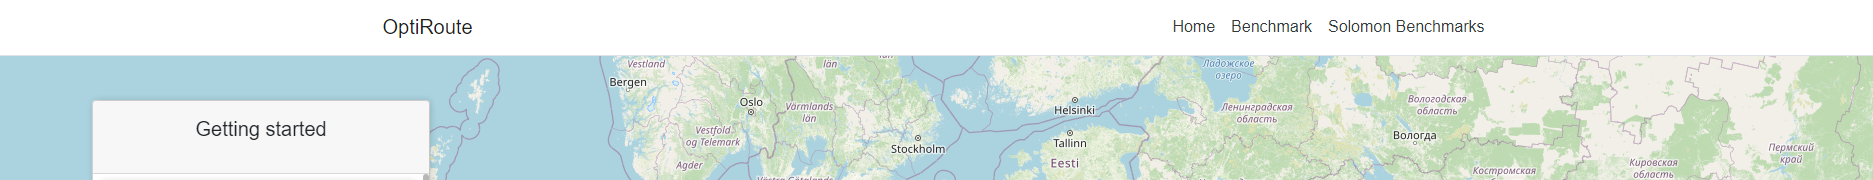
\includegraphics[width=\textwidth]{images/navbar.PNG}
\caption{Navigation bar}
\label{fig:navbar}
\end{figure}

The navigation bar (Fig. \ref{fig:navbar}) is visible at the top of every page in the application, it contains 3 buttons:
\begin{itemize}
\item Home - redirects to the home page.
\item Benchmark - redirects to a page where the user can upload the benchmark file and solve the problem found in the file.
\item Solomon Benchmarks - redirects to a page with a table comparing OptiRoute solutions and the best known solutions for Solomon benchmark instances.
\end{itemize}

\subsection{Home Page}
\begin{figure}[H]
\centering
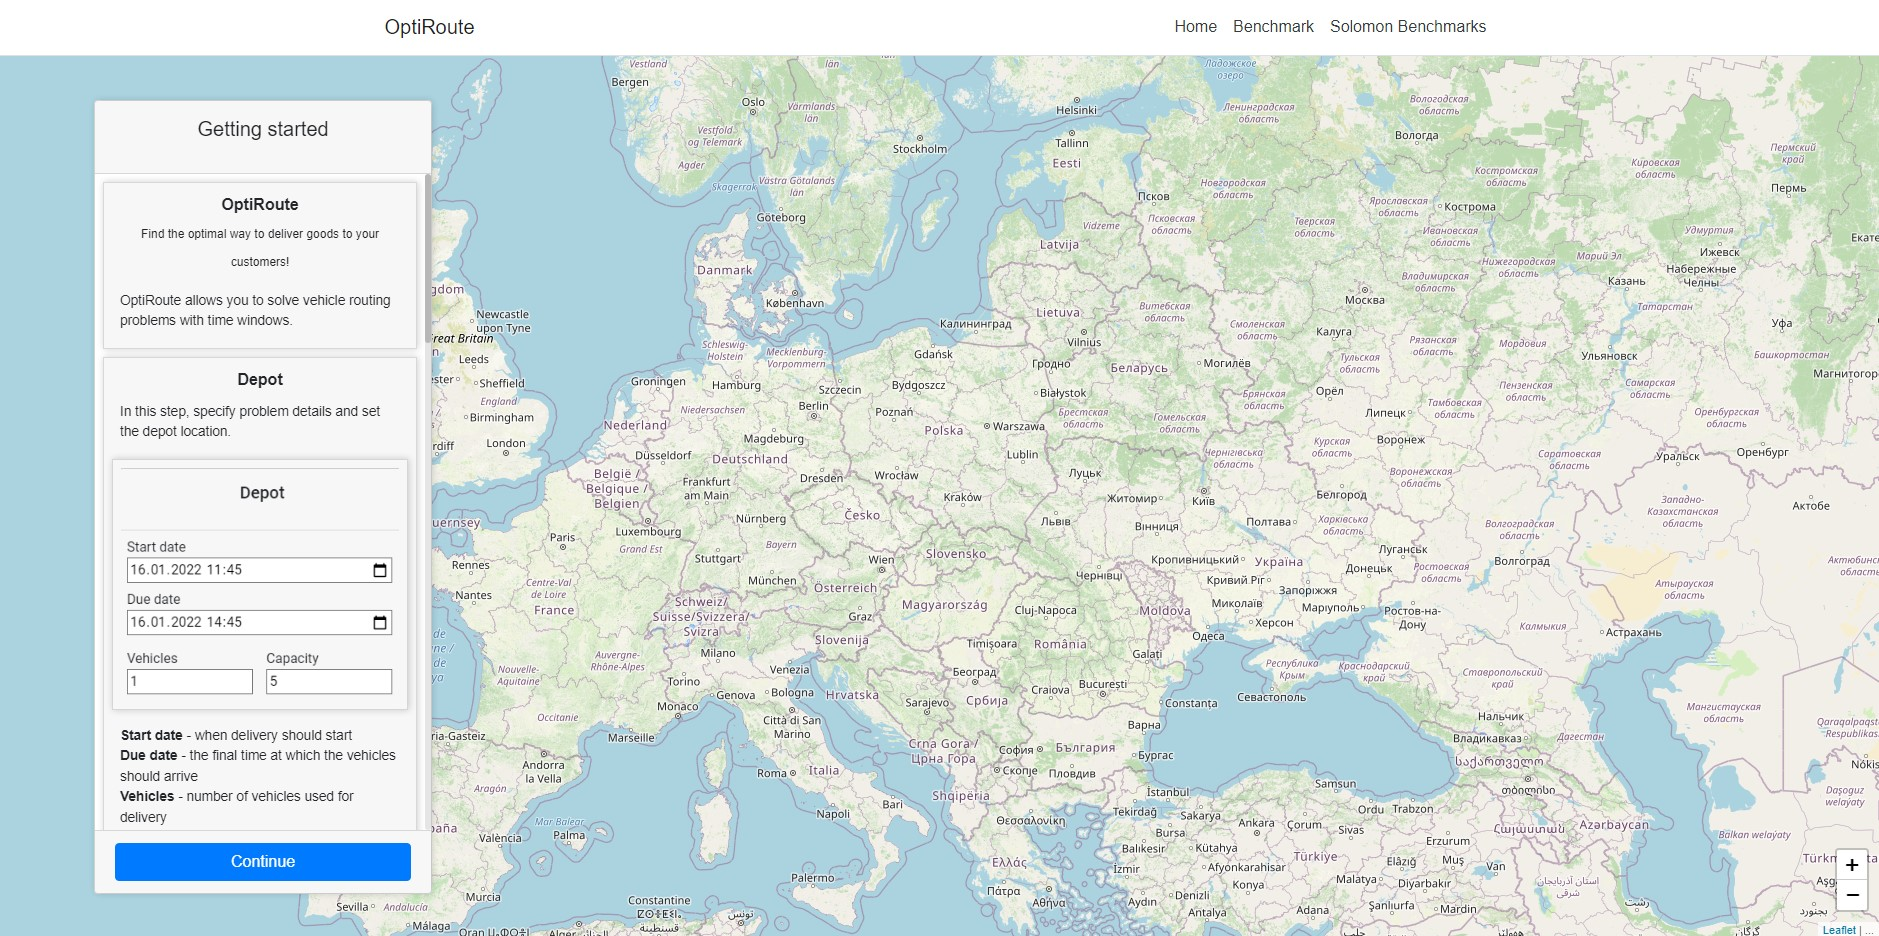
\includegraphics[width=\textwidth]{images/home.jpg}
\caption{Home page}
\label{fig:home}
\end{figure}

The home page (Fig. \ref{fig:home}) consist of map and the sidebar. The user can zoom in, zoom out, move freely around the map and add markers with a mouse click (Fig. \ref{fig:markers}). The sidebar consists of required inputs for data or details depending on the current step of the problem definition process.

\begin{figure}[H]
\centering
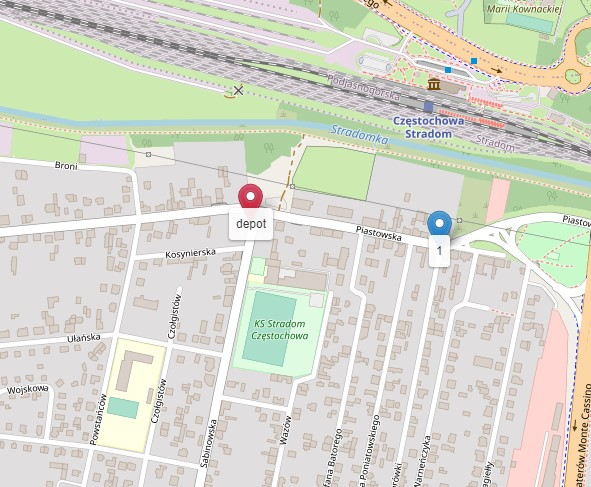
\includegraphics[scale=0.5]{images/markers.jpg}
\caption{Markers placed on the map}
\label{fig:markers}
\end{figure}

\subsection{Sidebar}
The sidebar is where the user can define the details of the problem as well as see the details of the solution. The whole process is divided into individual steps, so the content of the sidebar depends on which stage the user is currently at.
\subsubsection{Getting started}
\begin{figure}[H]
\centering
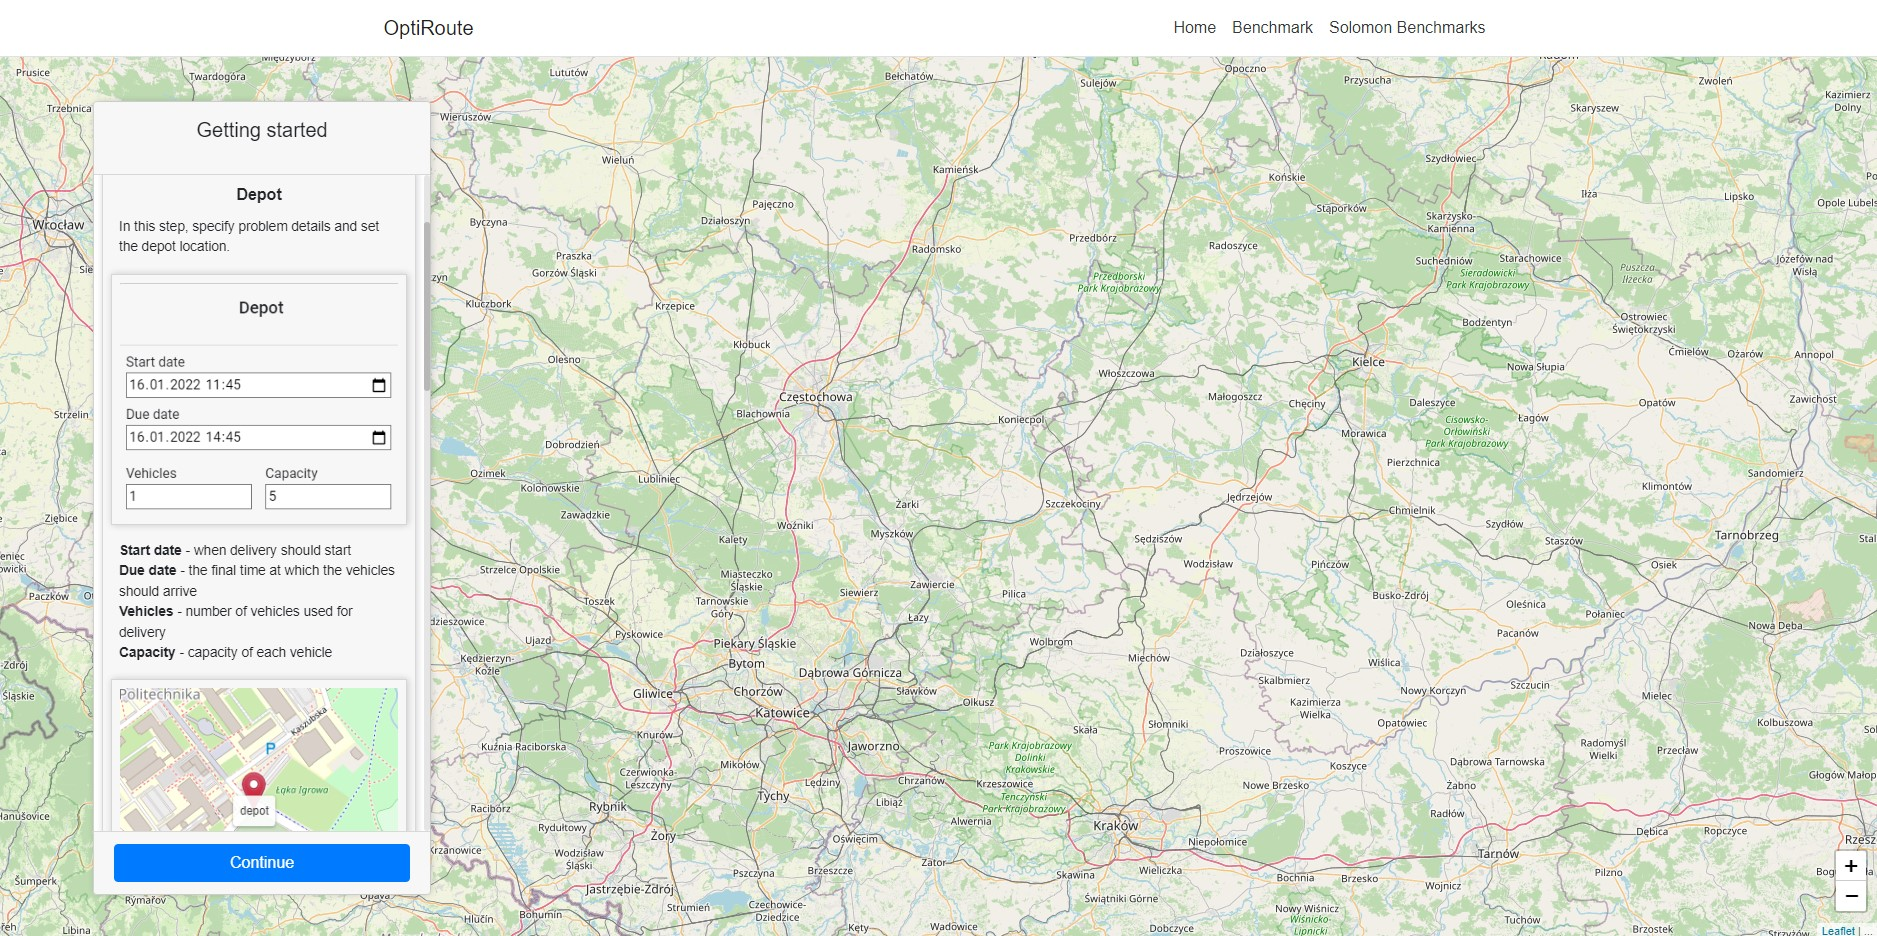
\includegraphics[width=\textwidth]{images/gettingStarted.jpg}
\caption{Getting started step in the sidebar}
\label{fig:gettingStarted}
\end{figure}
The "Getting Started" step in the sidebar (Fig. \ref{fig:gettingStarted}) provides a short user guide, explaining step-by-step how to use the application. Screenshots and short descriptions of the steps to follow make it easier for first-time users to use the app. After clicking the "Continue" button at the bottom of the sidebar, the contents of the sidebar will change to the "Depot" step.

\subsubsection{Depot}
In the "Depot" step, the user must place the depot marker by clicking on the desired location on the map and then specify the details in the input fields in the sidebar (Fig. \ref{fig:depot}).



At the bottom of the sidebar (Fig. \ref{fig:depot}) are two buttons, "Back" and "Continue", which allow the user to move on to the next step or return to the previous step.

\begin{figure}[H]
\centering
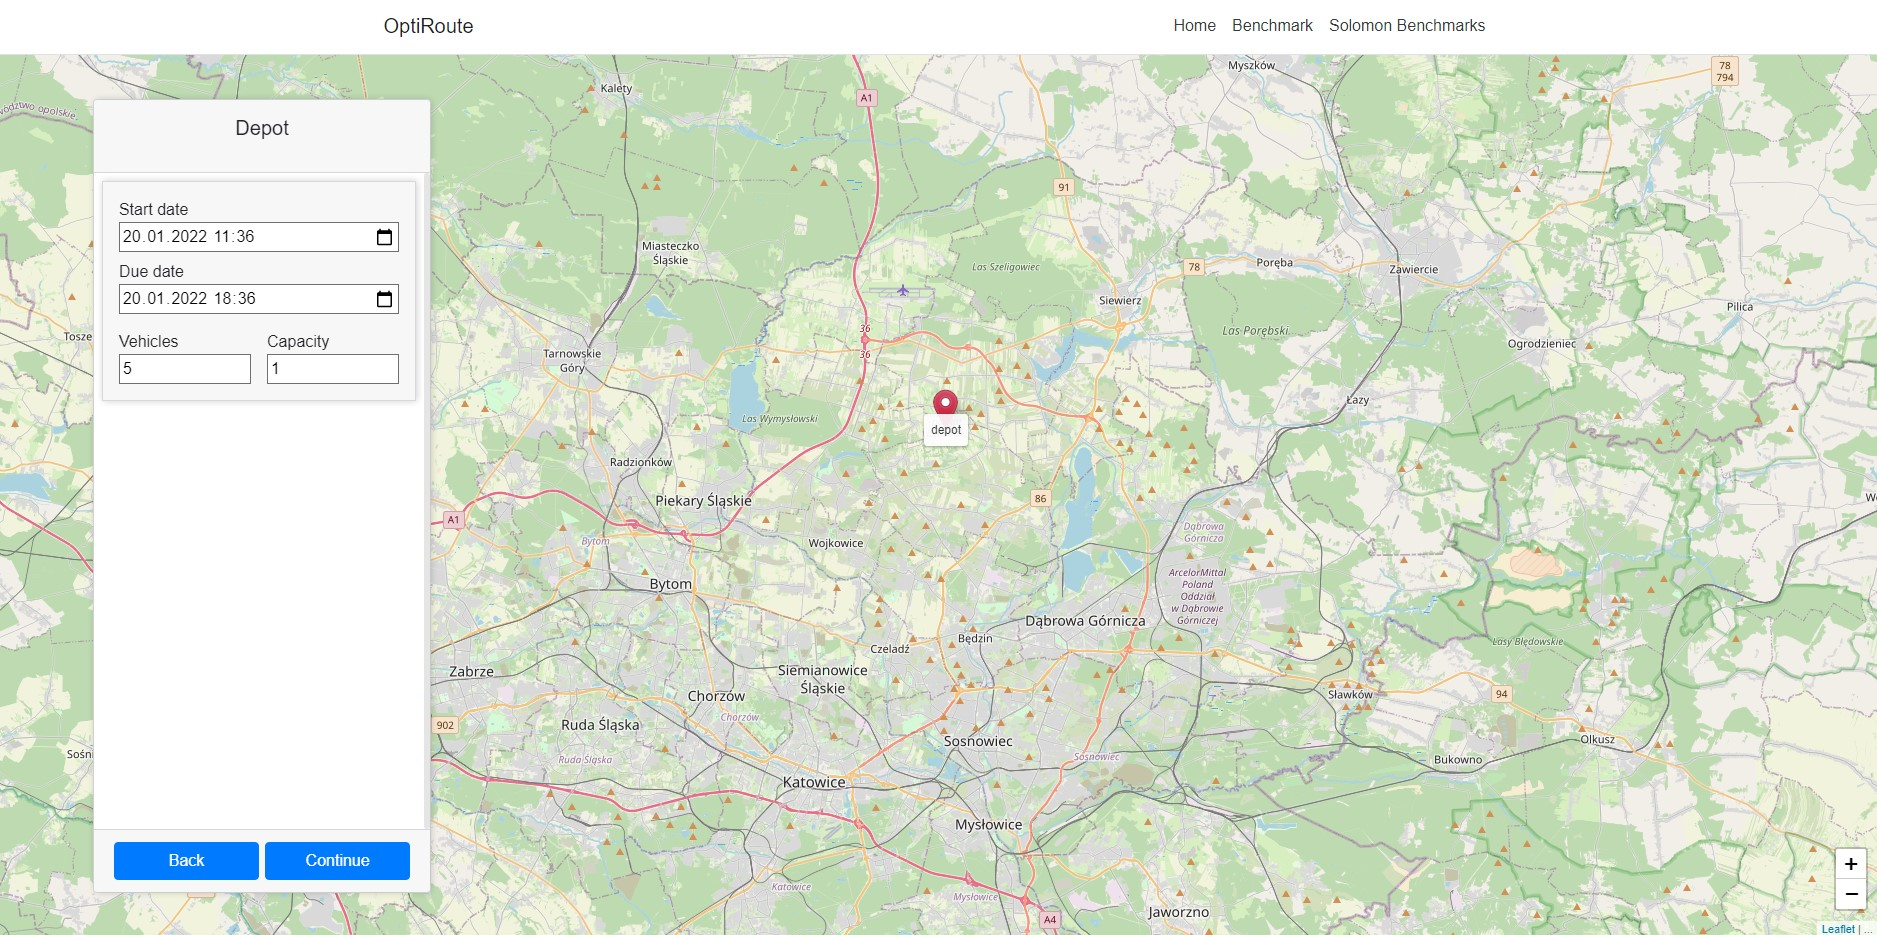
\includegraphics[width=\textwidth]{images/depot.jpg}
\caption{Depot step}
\label{fig:depot}
\end{figure}

The "Depot" form (Fig. \ref{fig:depot}) contains input fields:
\begin{itemize}
    \item Start date - time when the delivery should start.
    \item Due date - the final time at which the vehicles should arrive at the depot.
    \item Vehicles - number of vehicles used for delivery.
    \item Capacity - the capacity of each vehicle.
\end{itemize}



The validation rules applied to the input data:
\begin{itemize}
    \item Start date - is required and cannot be greater than or equal to the Due date.
    \item Due date - is required and cannot be less than or equal to the Start date.
    \item Vehicles - is required and must be an integer.
    \item Capacity - is required and must be an integer.
\end{itemize}
When the input data is invalid it will display appropriate message and disable the "Continue" button, preventing the user from proceeding to the next step (Fig. \ref{fig:invalidDepot}). The "Continue" button will also be inactive if the depot marker is not placed on the map.
\begin{figure}[H]
\centering
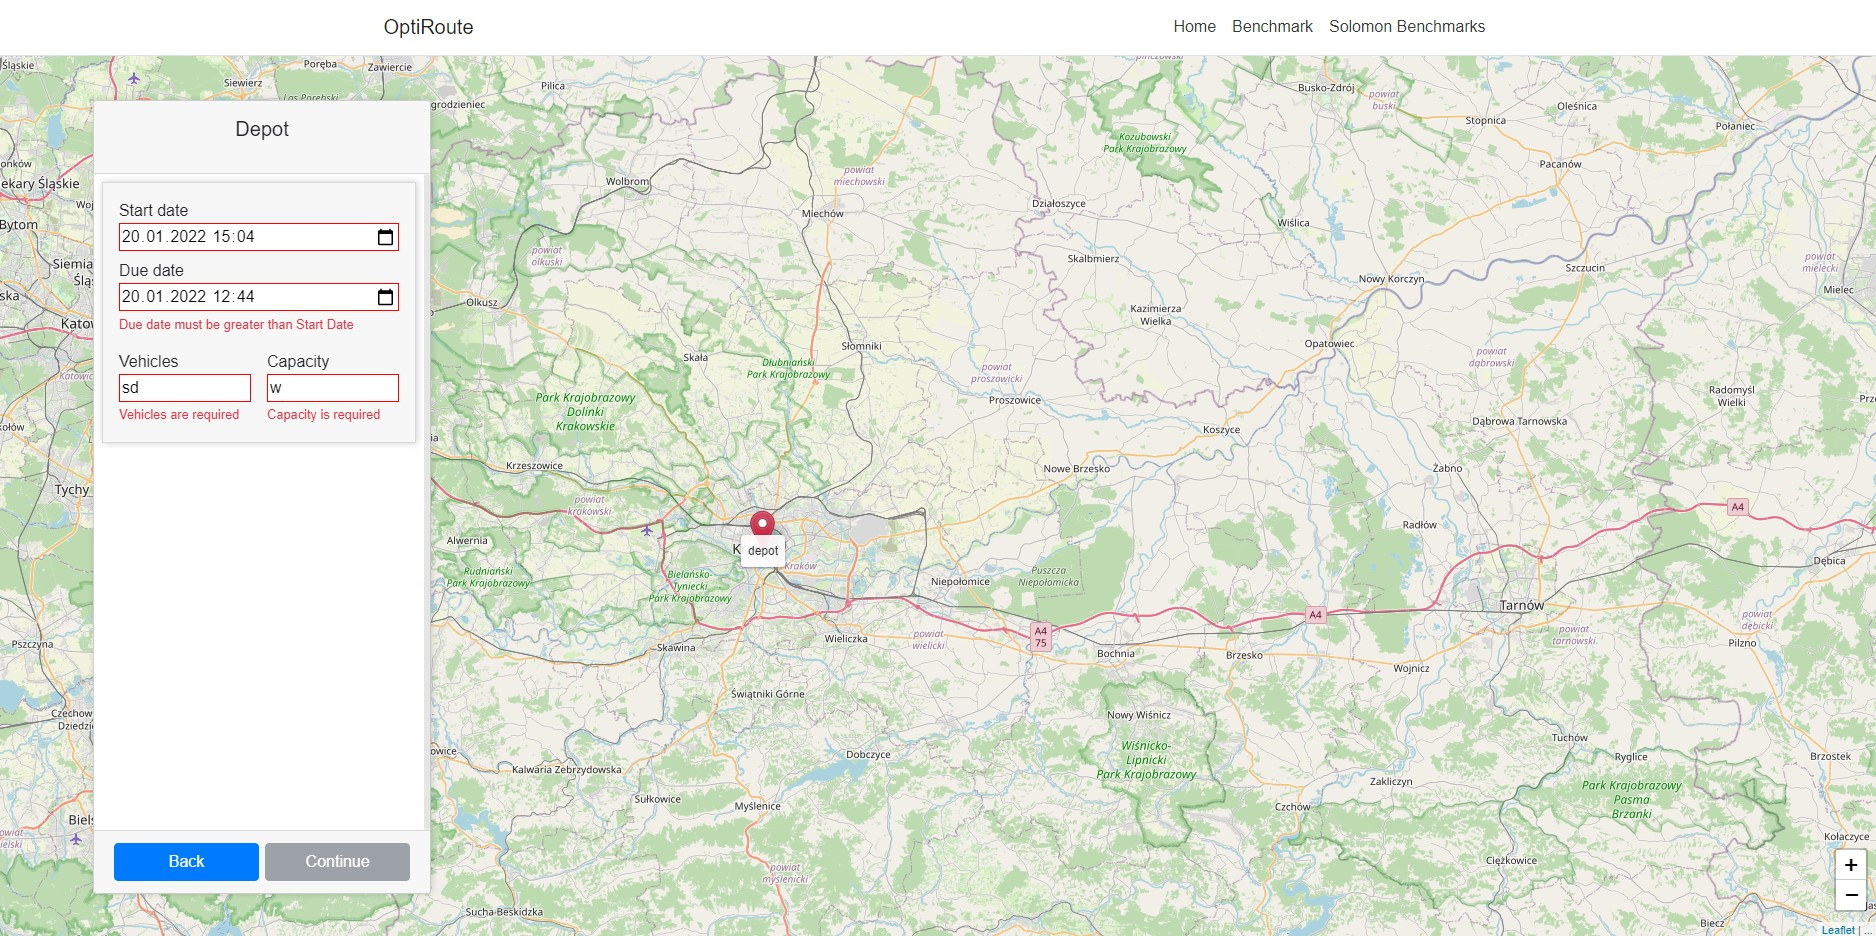
\includegraphics[width=\textwidth]{images/invalidDepot.jpg}
\caption{Depot form with invalid data}
\label{fig:invalidDepot}
\end{figure}



\subsubsection{Customers}

The 'Customers' section allows the user to place customer markers on the map and specify the details of each customer. Customer markers are placed in the same way as depot markers. When a location is selected, a separate section for that customer will appear in the sidebar, marked with the customer number in the left corner (Fig. \ref{fig:customers}). 



At the bottom of the sidebar (Fig. \ref{fig:customers}) there are two buttons, "Back" and "Solve", which allow the user to solve the problem and go to the presentation of the results or return to the "Depot" step.

\begin{figure}[H]
\centering
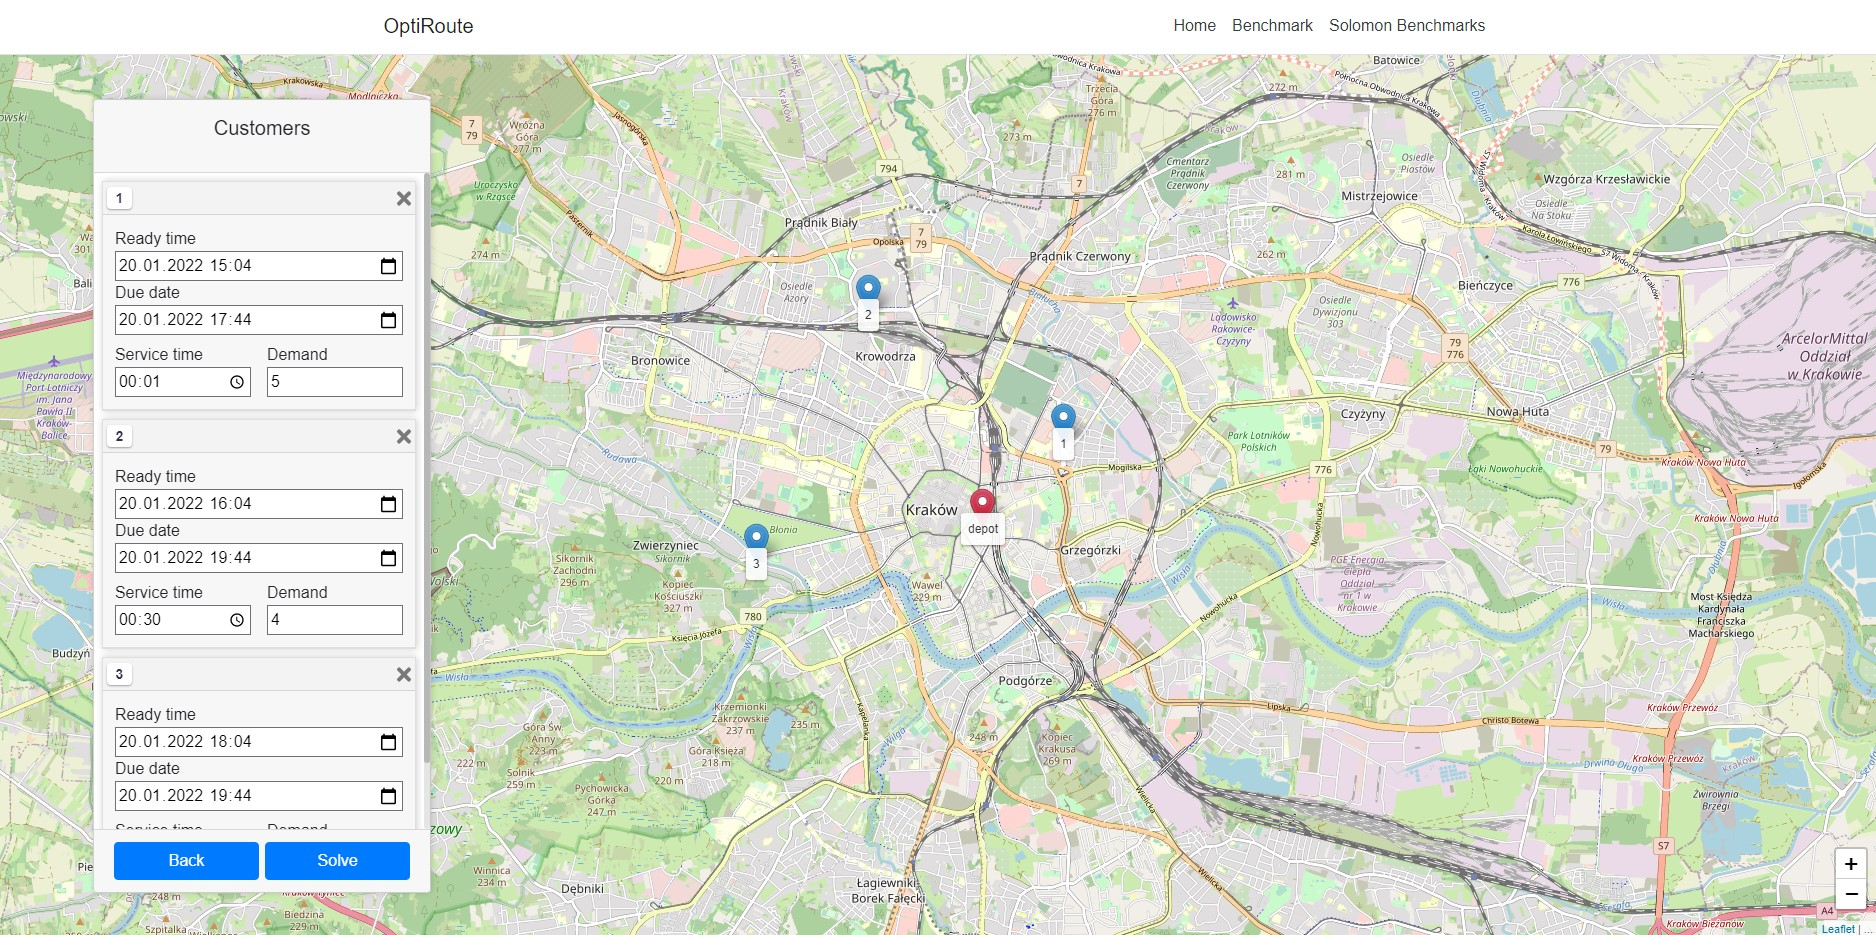
\includegraphics[width=\textwidth]{images/customers.jpg}
\caption{Customers step}
\label{fig:customers}
\end{figure}

Each customer form (Fig. \ref{fig:customers}) contains input fields:
\begin{itemize}
    \item Ready time - the earliest date on which the customer can take delivery.
    \item Due date - final date on which the customer may take delivery.
    \item Service time - time taken to accept delivery.
    \item Demand - quantity of goods in delivery.
\end{itemize}



The validation rules applied to the input data:
\begin{itemize}
    \item Ready time - is required, cannot be greater than or equal to the Due date and must be within the depot time window.
    \item Due date - is required, cannot be less than or equal to the Ready time and must be within the depot time window.
    \item Service time - is required.
    \item Demand - is required and must greater than 0.
\end{itemize}

As with the "Depot" form, when the data entered is invalid, it will display appropriate message and disable the "Solve" button, preventing the user from solving the problem (Fig. \ref{fig:invalidCustomers}). The "Solve" button will also be inactive if there are no customers.

\begin{figure}[H]
\centering
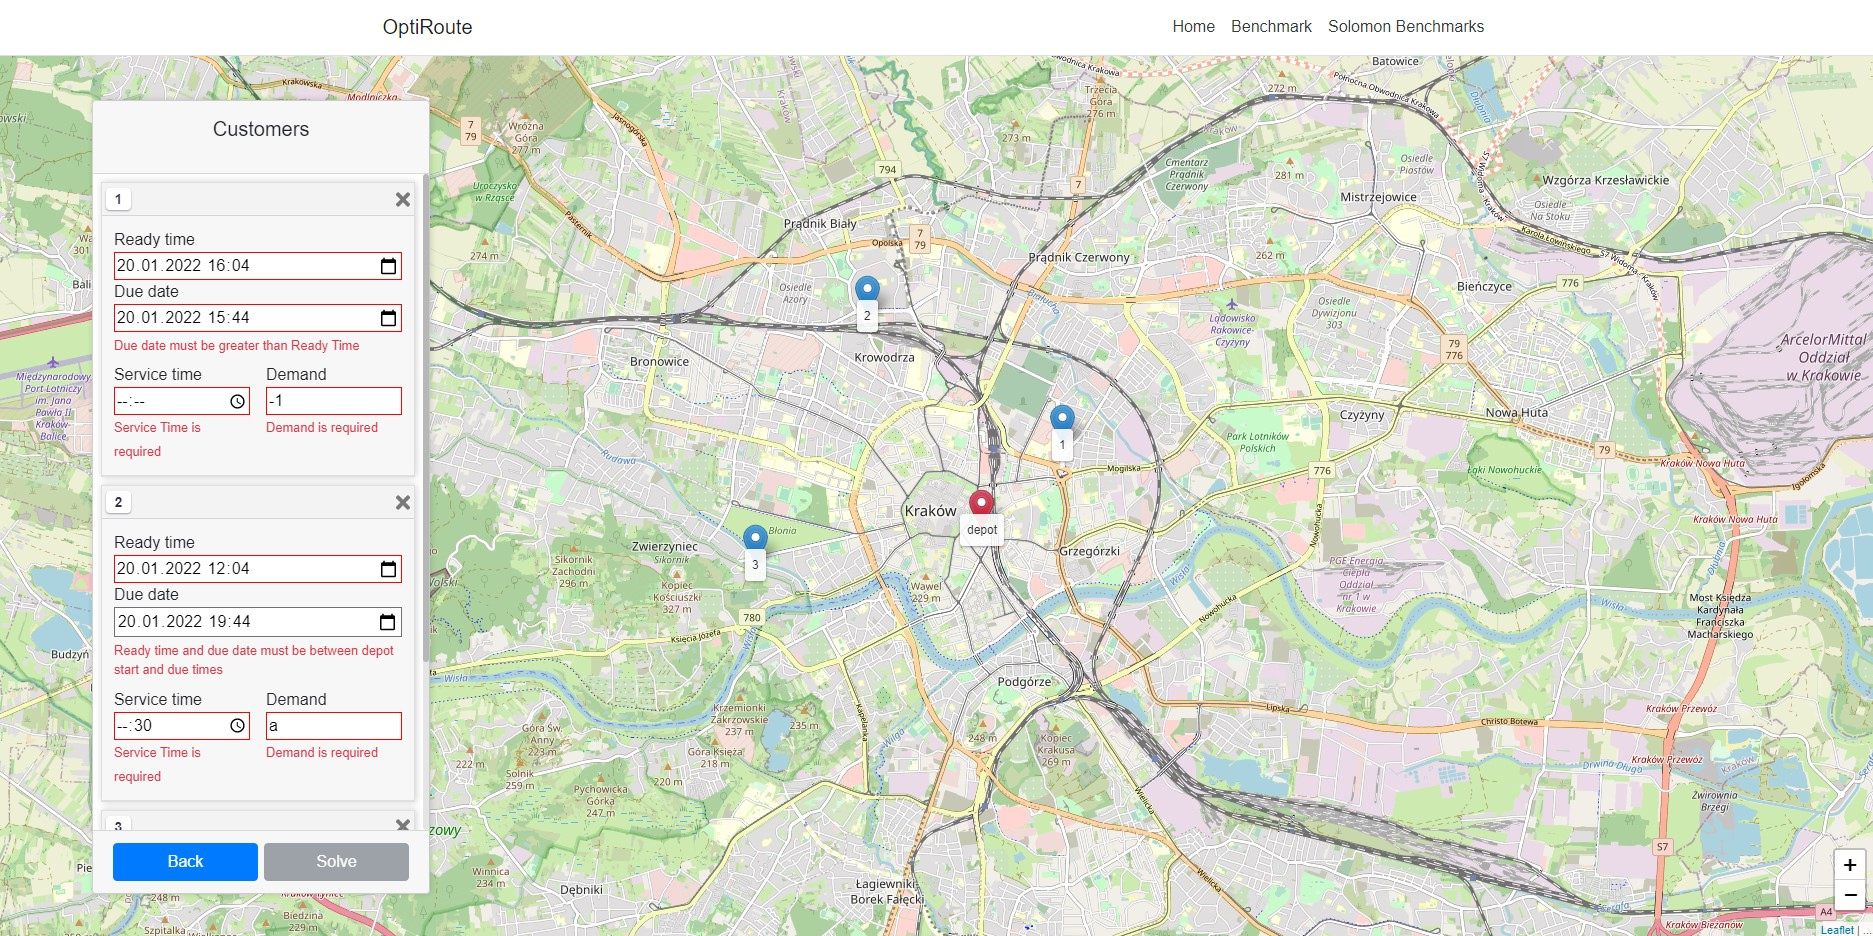
\includegraphics[width=\textwidth]{images/invalidCustomers.jpg}
\caption{Customers forms with invalid data}
\label{fig:invalidCustomers}
\end{figure}

\subsubsection{Solution}
When the problem is feasible the solution (routes) is drawn on the map, and the details of the entire solution and each route are shown in the sidebar (Fig \ref{fig:solution}).



At the bottom of the sidebar (Fig. \ref{fig:solution}) there is "Back" button which allows the user to clear the routes from the map and come back to the previous step.

\begin{figure}[H]
\centering
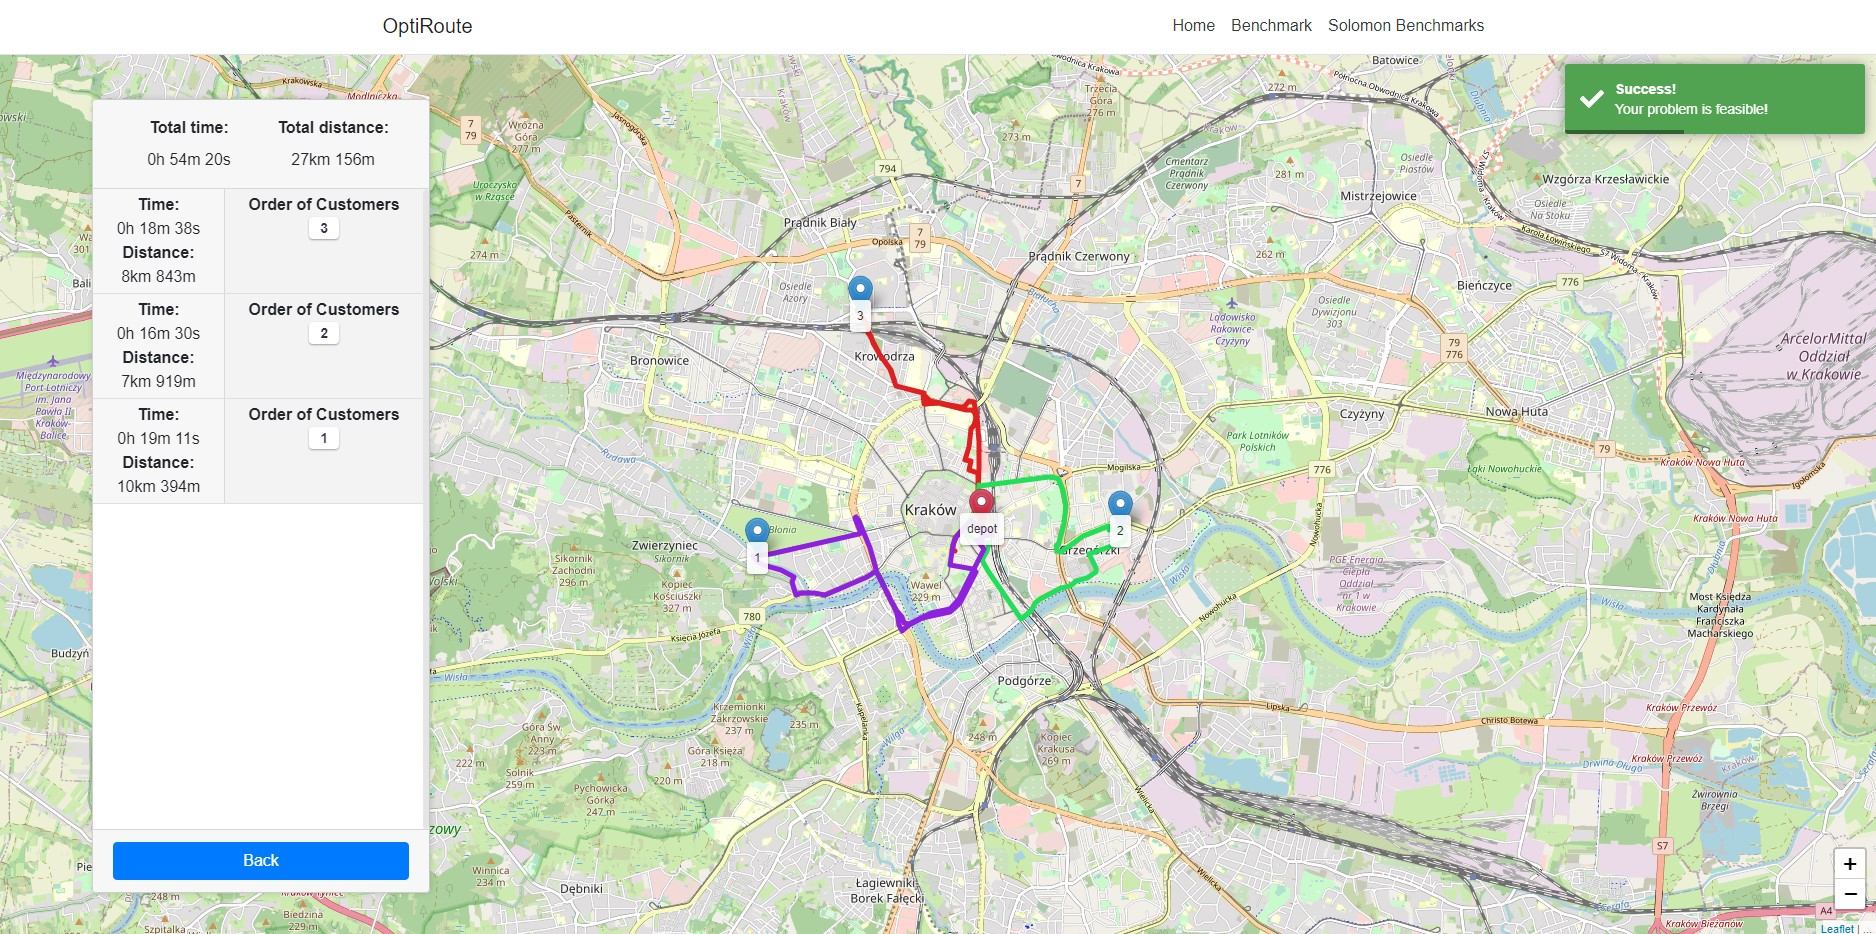
\includegraphics[width=\textwidth]{images/solution.jpg}
\caption{Solution}
\label{fig:solution}
\end{figure}

The user can highlight one of the routes on the map by hovering the mouse over the route details in the sidebar (Fig. \ref{fig:solutionHover}).

\begin{figure}[H]
\centering
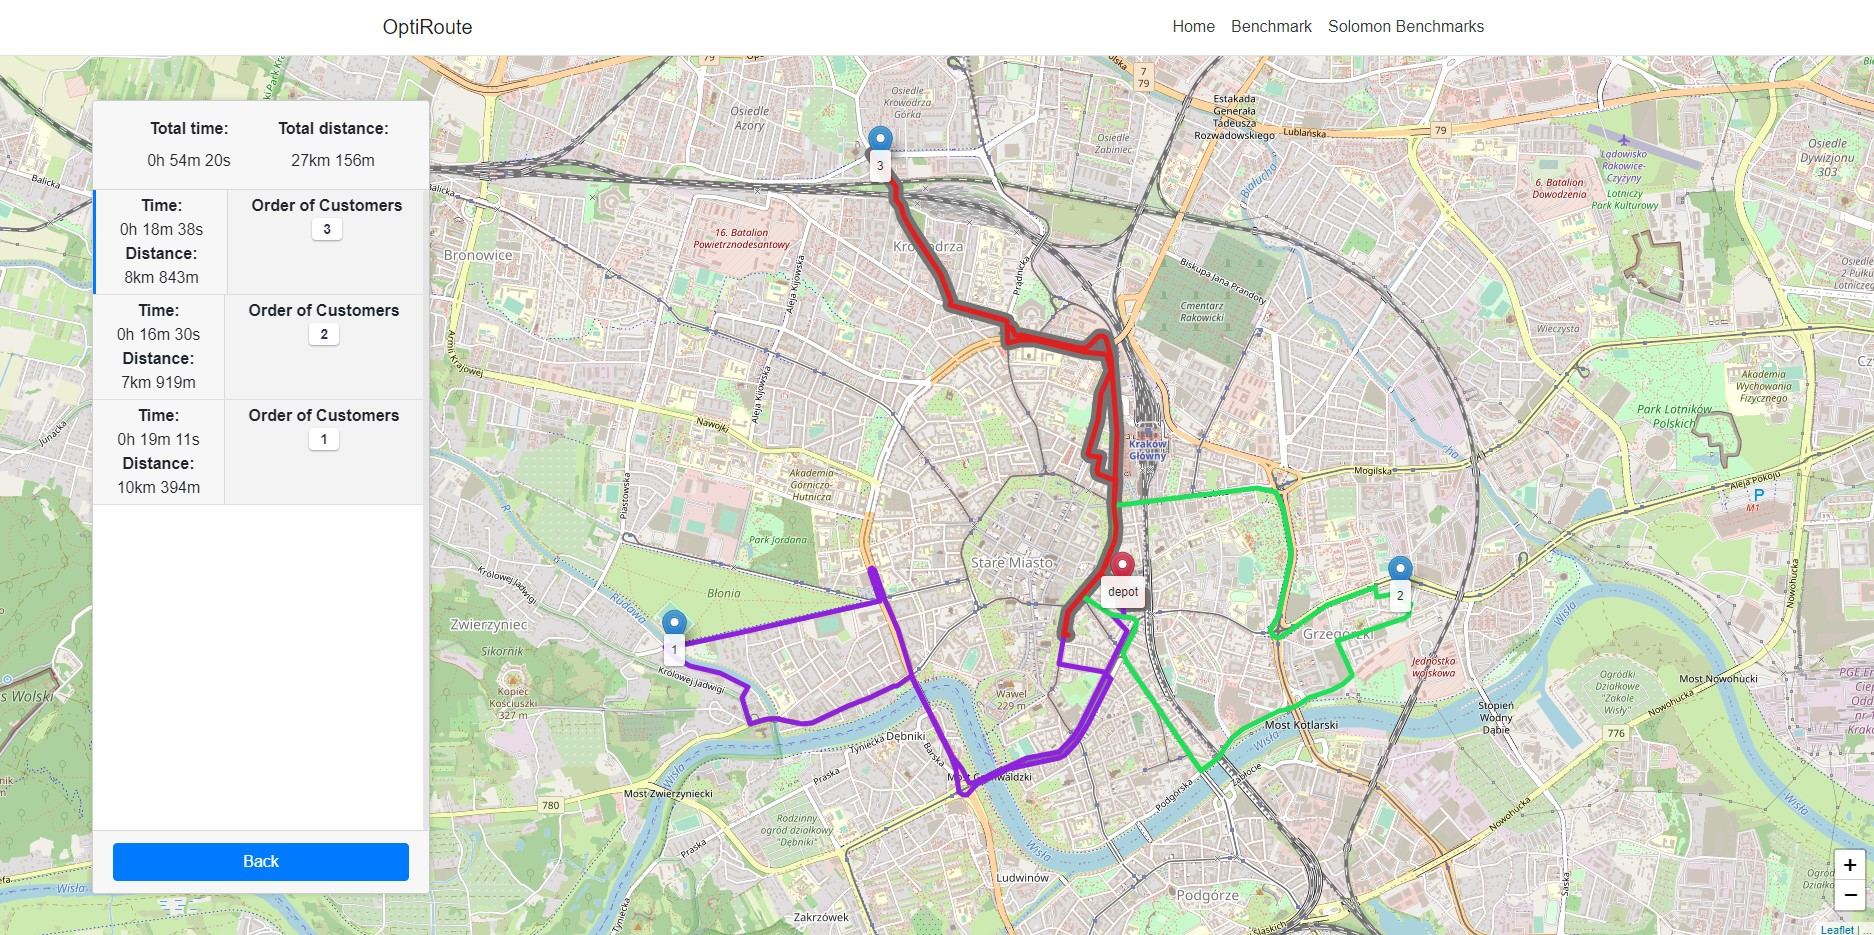
\includegraphics[width=\textwidth]{images/solutionHover.jpg}
\caption{Highlighted route}
\label{fig:solutionHover}
\end{figure}

\subsection{Benchmark}

The "Benchmark" page (Fig. \ref{fig:benchmark}) allows the user to solve a problem contained in a benchmark file. This file must be in .txt format and must match the Solomon Benchmark instance file structure \cite{bib:sintefDocumentation}. The "solve" button sends the problem to the backend server. If the format of the selected file is invalid, a message is displayed informing the user about the problem(Fig. \ref{fig:benchmarkInvalidFormat}). If the loaded text file does not match the Solomon Benchmark structure, a message is returned indicating the line where the validation error occurred (Fig. \ref{fig:benchmarkInvalidFile}).  When the file is successfully solved, the solution details are displayed along with a button to visualise the solution on the image (Fig. \ref{fig:benchmarkSolved}).

\begin{figure}[H]
\centering
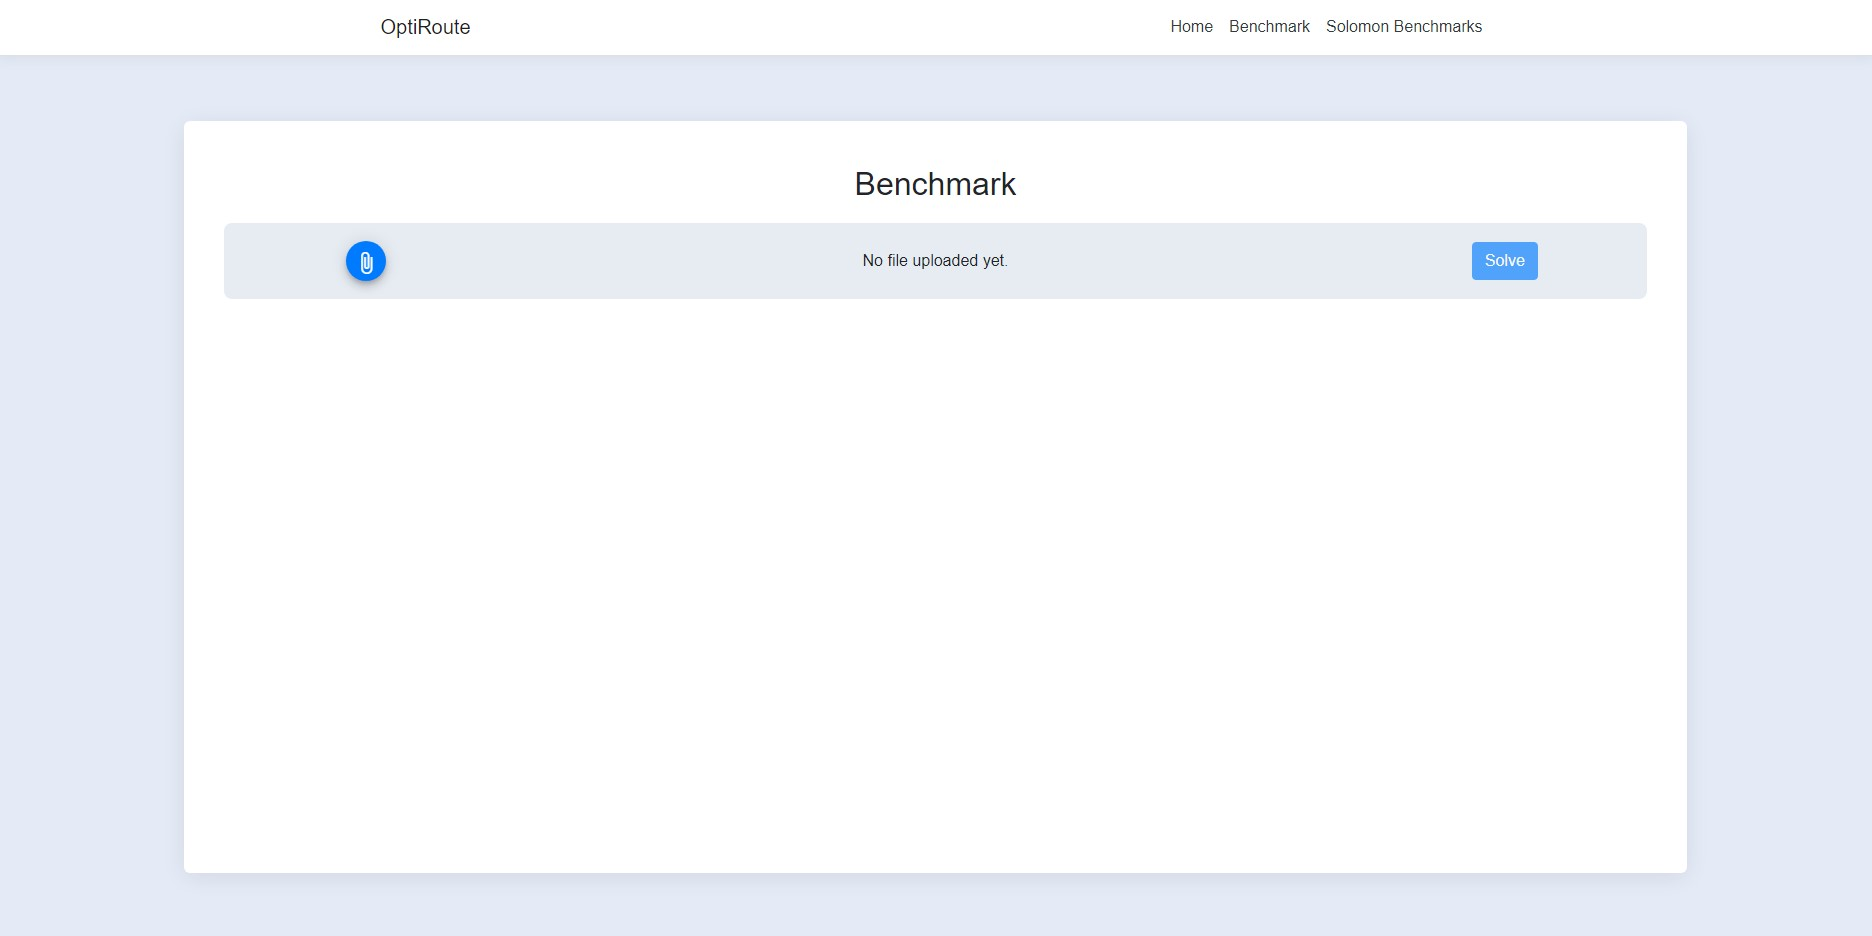
\includegraphics[width=\textwidth]{images/benchmark.jpg}
\caption{Benchmark page}
\label{fig:benchmark}
\end{figure}

\begin{figure}[H]
\centering
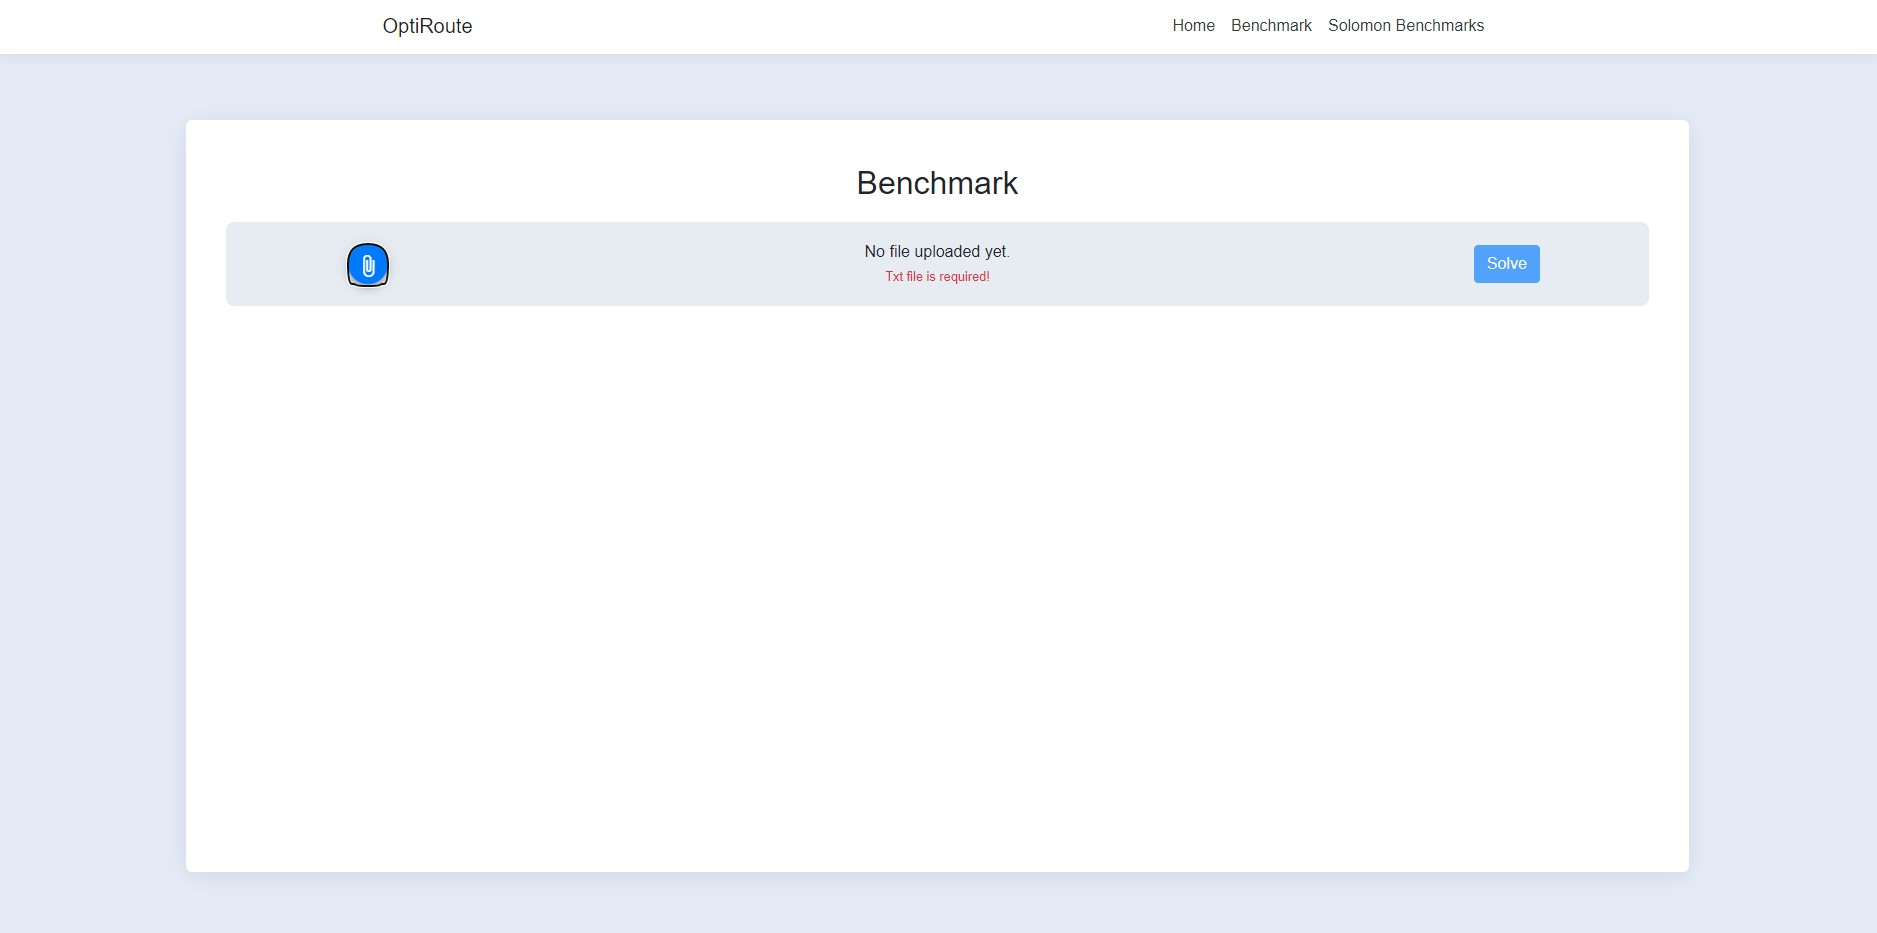
\includegraphics[width=\textwidth]{images/benchmarkInvalidFormat.jpg}
\caption{Invalid benchmark file format}
\label{fig:benchmarkInvalidFormat}
\end{figure}

\begin{figure}[H]
\centering
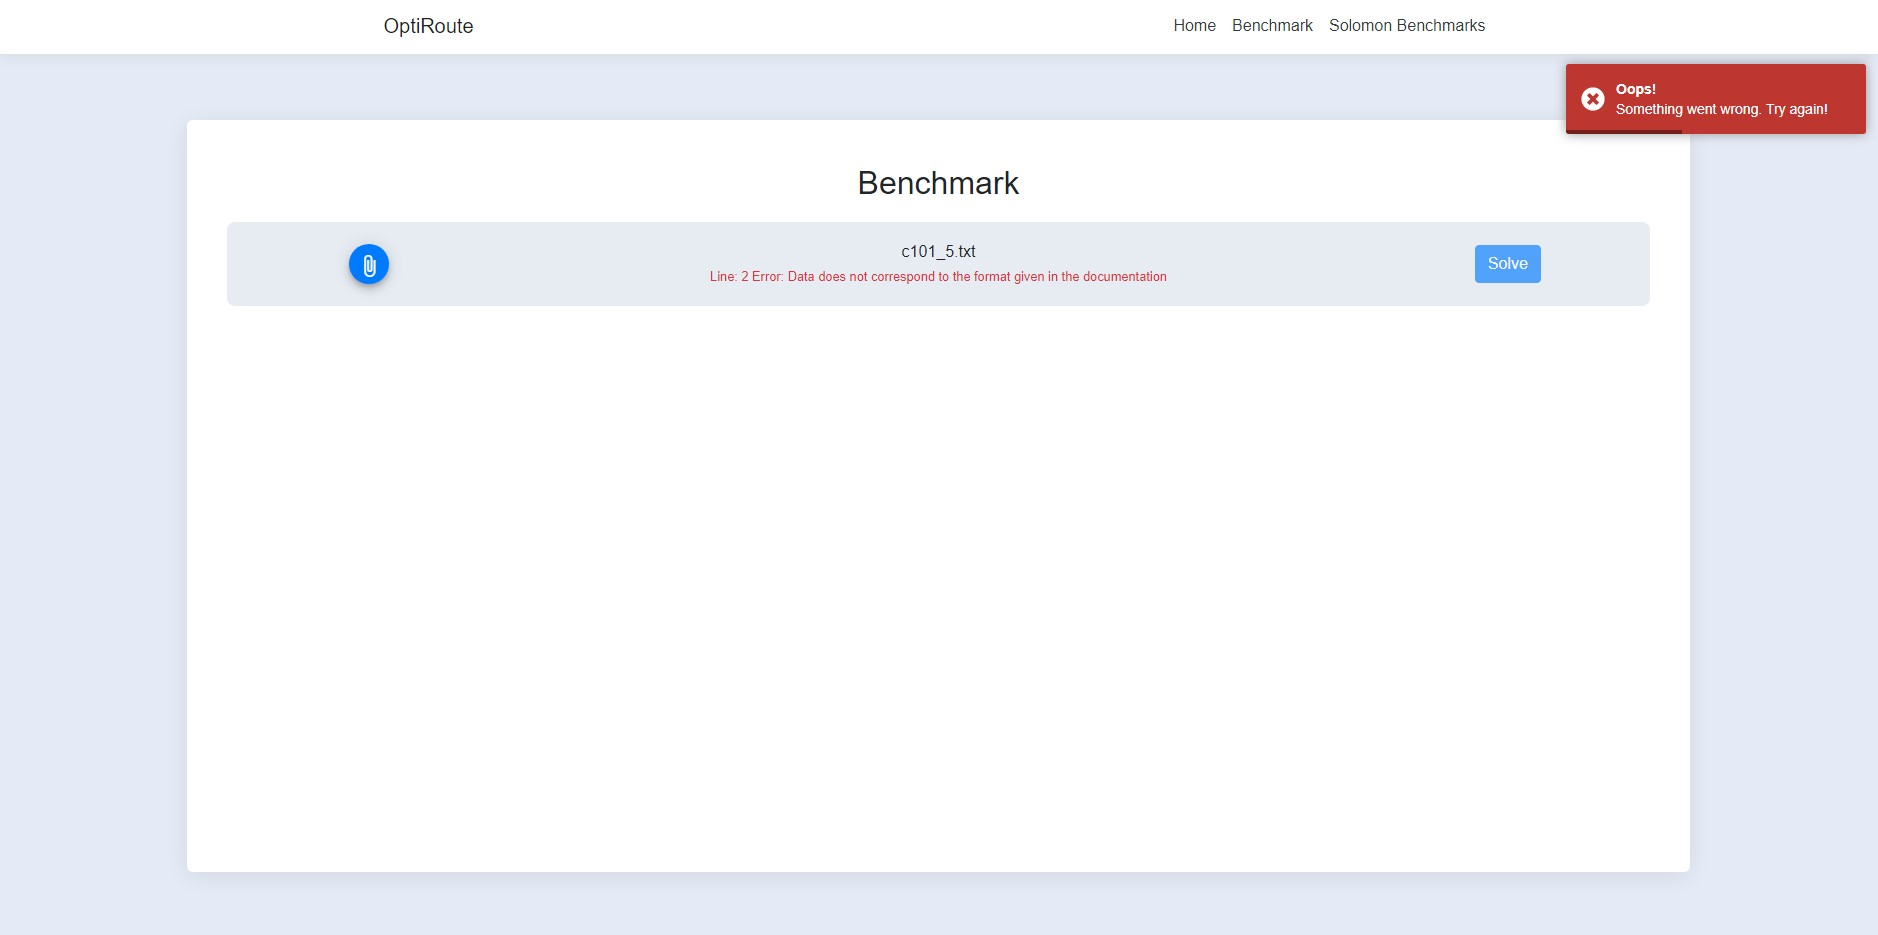
\includegraphics[width=\textwidth]{images/benchmarkInvalidFile.jpg}
\caption{Benchmark file validation error}
\label{fig:benchmarkInvalidFile}
\end{figure}

\begin{figure}[H]
\centering
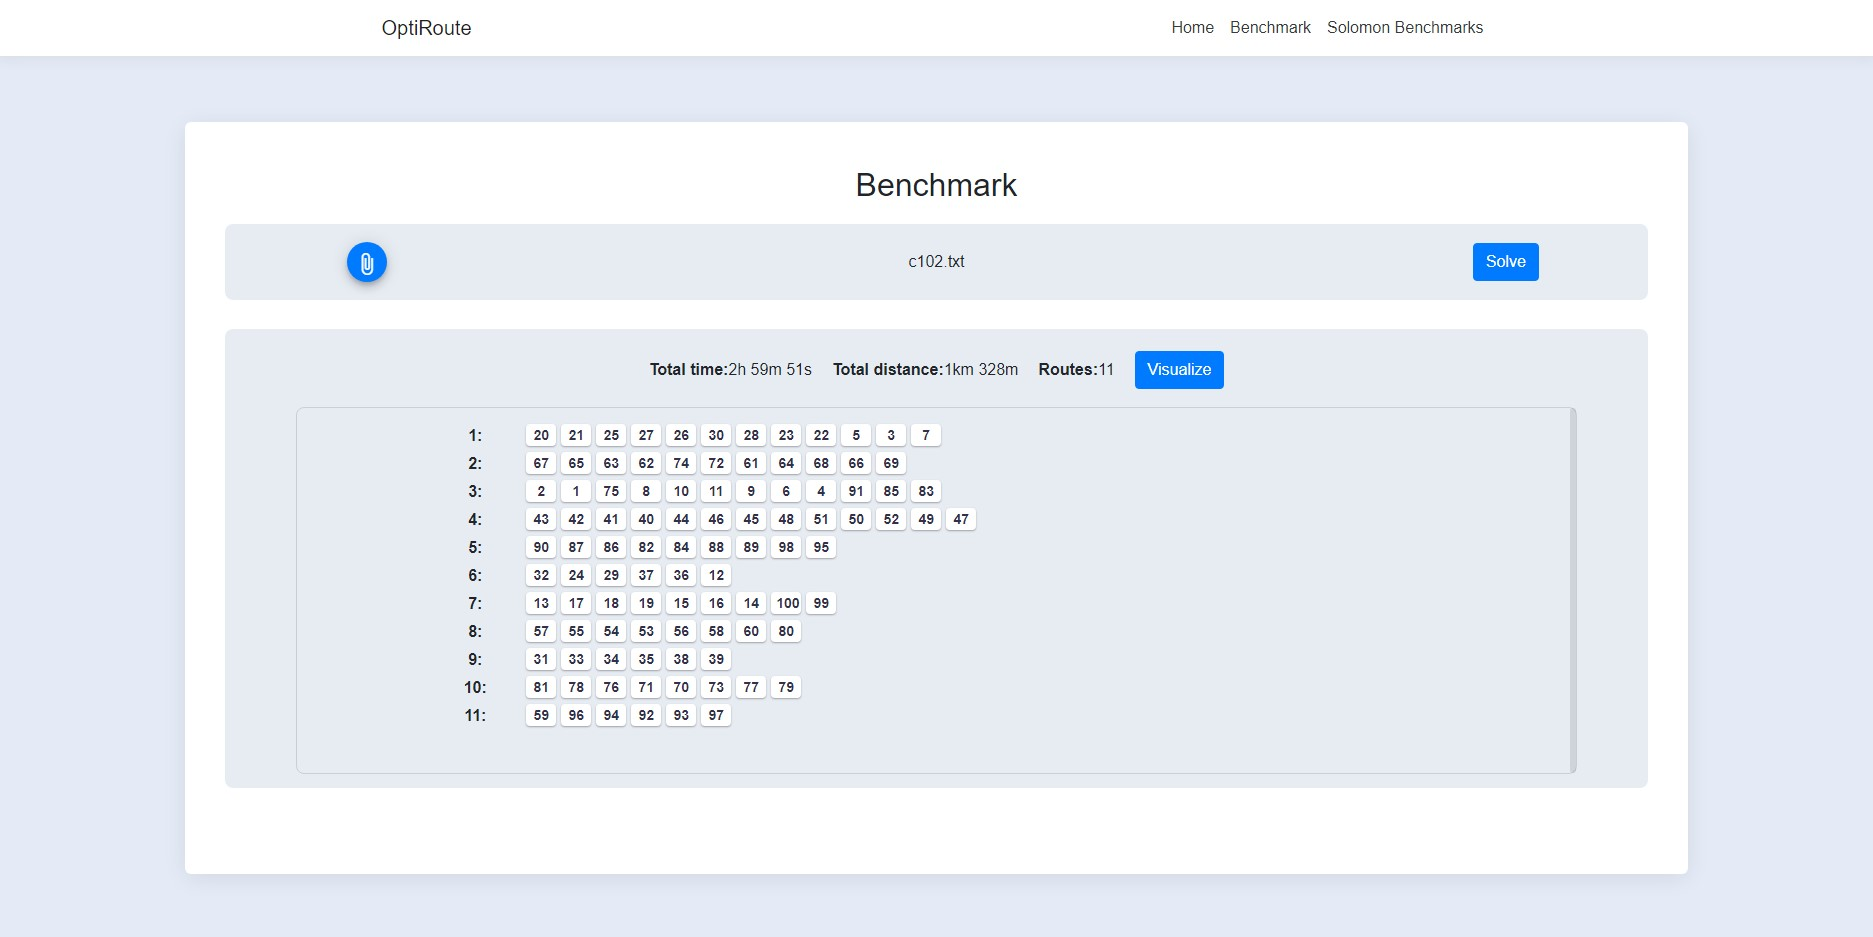
\includegraphics[width=\textwidth]{images/benchmarkSolved.jpg}
\caption{Details of the benchmark solution}
\label{fig:benchmarkSolved}
\end{figure}

\subsection{Solomon Benchmarks}

The "Solomon Benchmarks" page contains a table with the best known solutions and the solutions generated by the application for the Solomon benchmark problem instances (Fig. \ref{fig:solomonBenchmark}). The user can compare the "OptiRoute" solutions for each instance with the best solution. The table can be sorted and contains 6 pages with 10 records on each page (56 in total). Each row has two buttons "OptiRoute" and "Best", which allow the user to visualise the solutions of the current row on the image.

\begin{figure}[H]
\centering
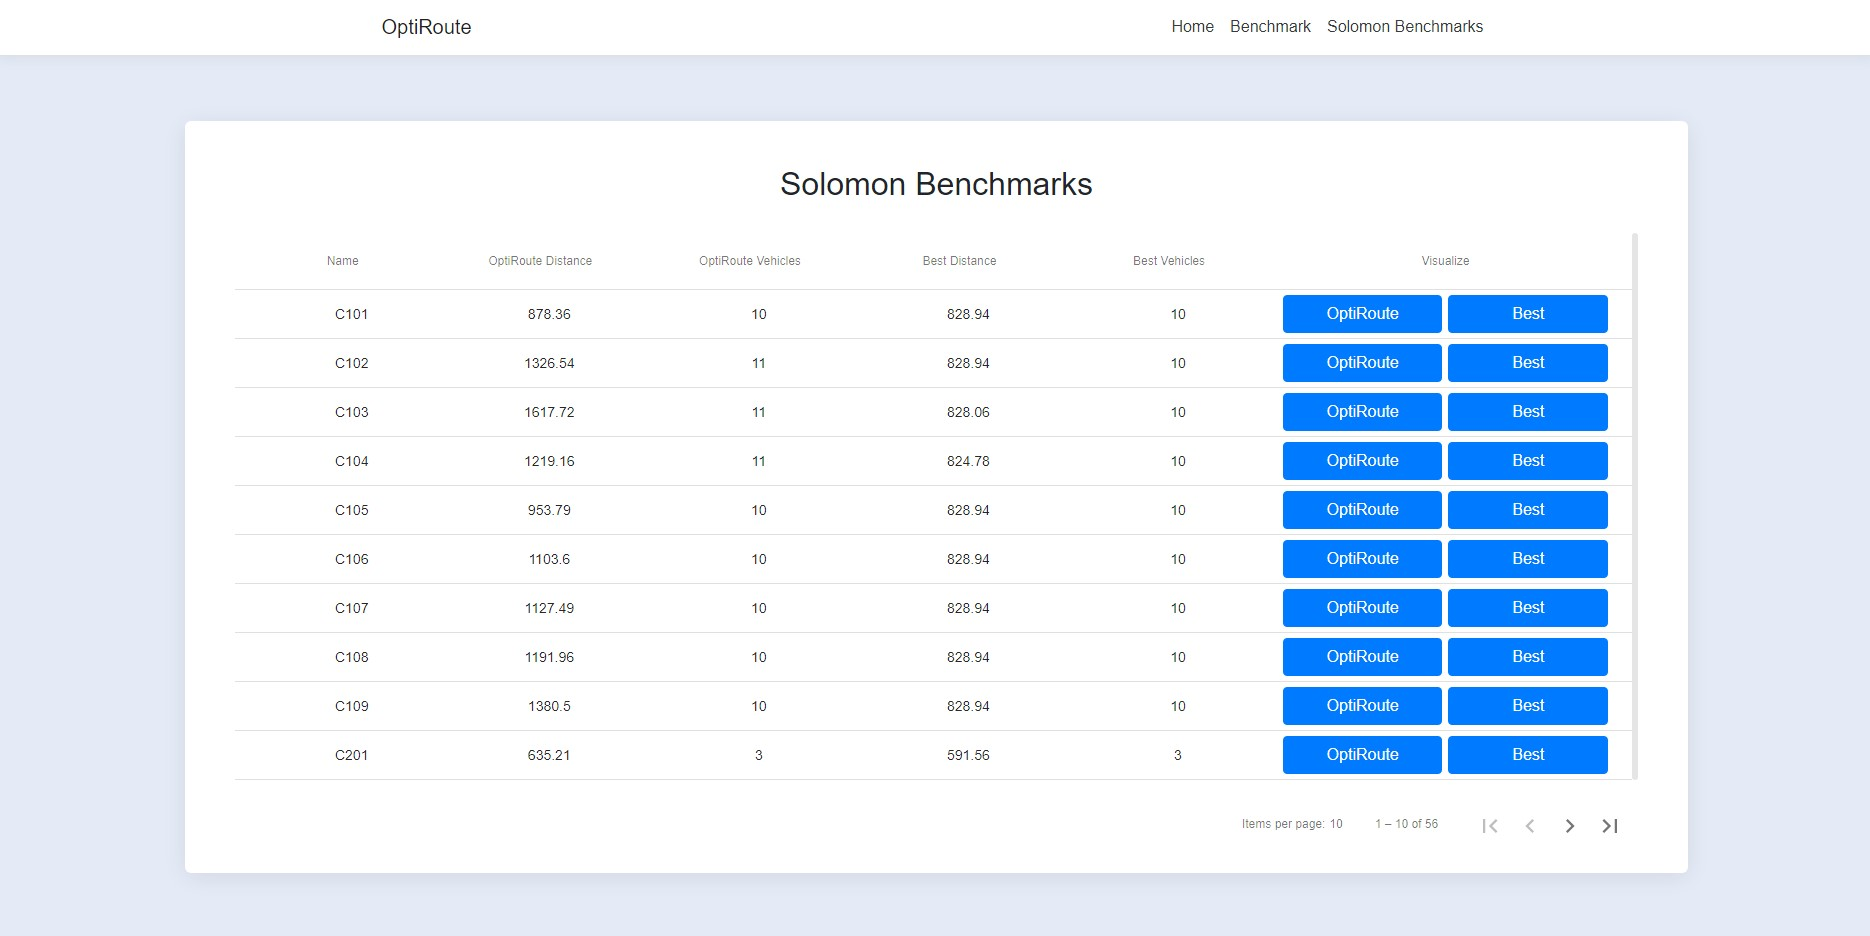
\includegraphics[width=\textwidth]{images/solomonBenchmark.jpg}
\caption{Solomon Benchmarks page}
\label{fig:solomonBenchmark}
\end{figure}

\subsection{Visualization}

The "Visualisation" dialog, as mentioned earlier, can be displayed on the "Benchmark" and "Solomon Benchmarks" pages by clicking the appropriate button. 

It contains a simple visualisation of the solution to the selected problem. Each customer is represented by a dot, customers belonging to the same route are connected by lines and have the same colour (Fig. \ref{fig:visualization}).

\begin{figure}[H]
\centering
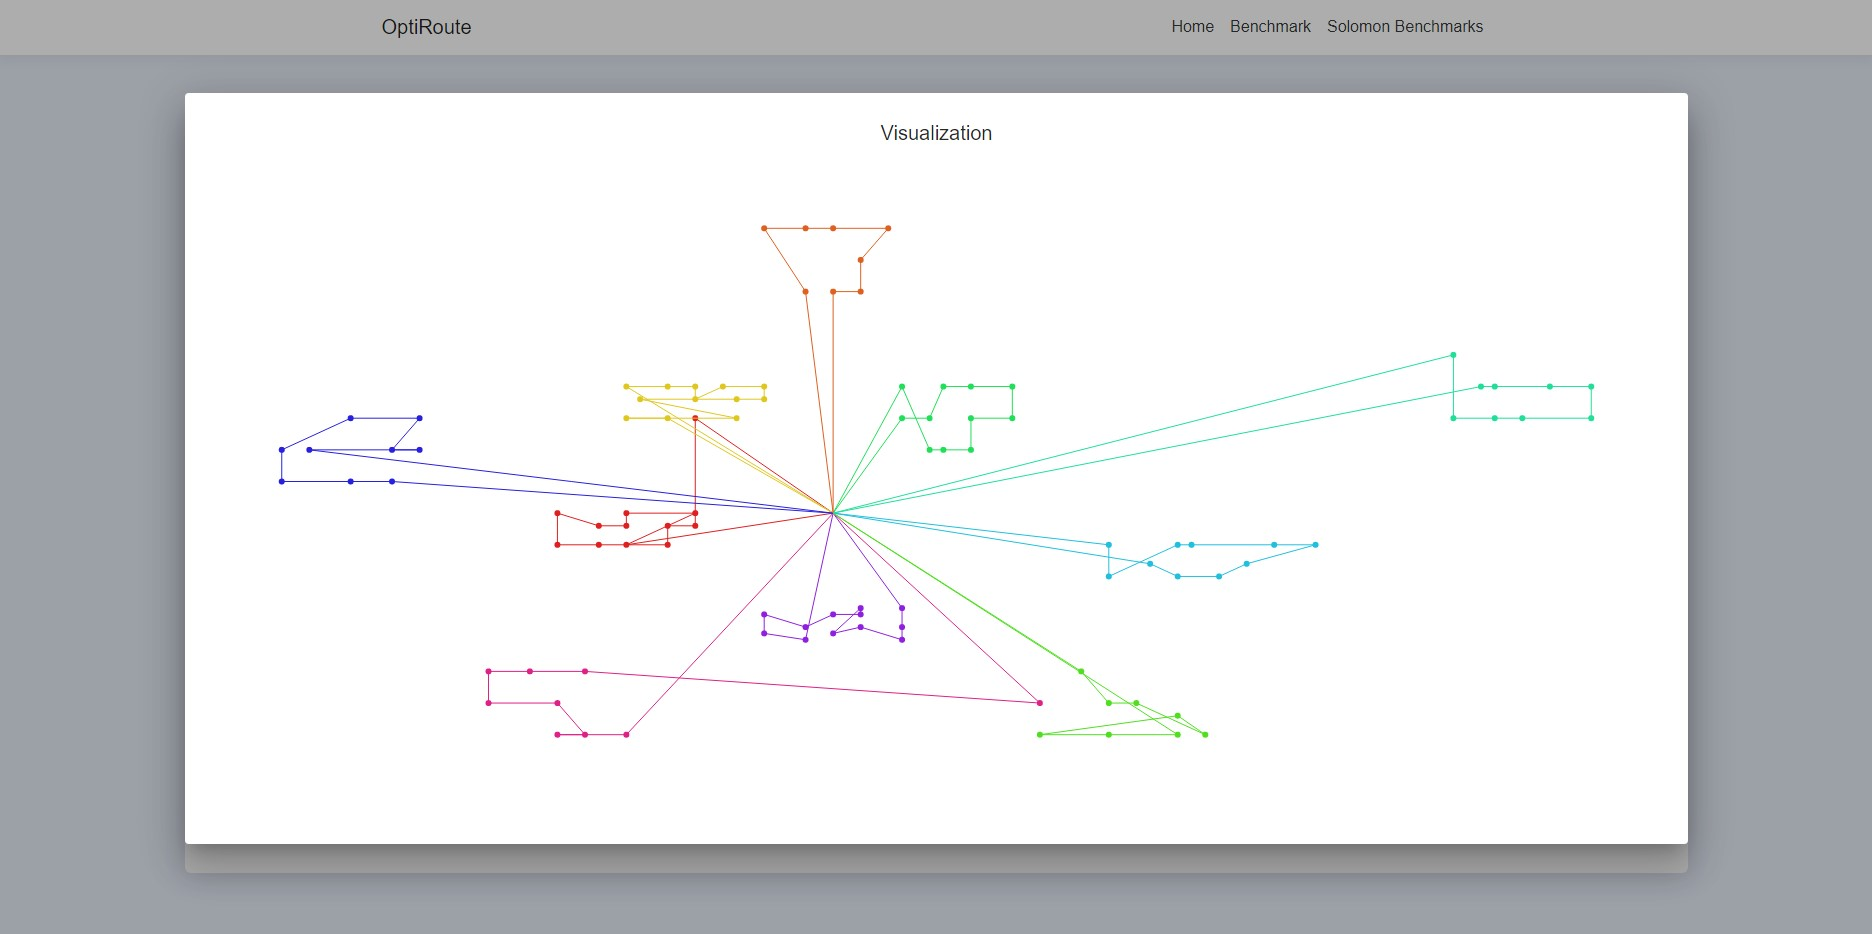
\includegraphics[width=\textwidth]{images/visualization.jpg}
\caption{Visualization dialog}
\label{fig:visualization}
\end{figure}

\subsection{Error}

If an unexpected error occurs, a corresponding message is displayed in the top right corner of the page (Fig. \ref{fig:error}). After a short time, the entire page reloads and is ready to be used again.

\begin{figure}[H]
\centering
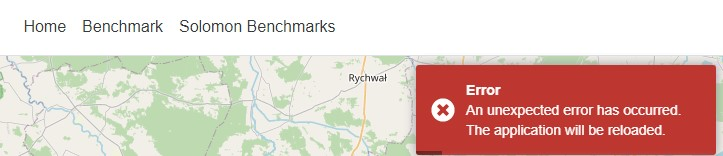
\includegraphics[scale=0.7]{images/error.jpg}
\caption{Error message}
\label{fig:error}
\end{figure}


\section{Security issues}
The application is intended to be accessible to any user, so no authentication or authorisation functions have been implemented in it. Therefore, no user security issues were encountered during the development of the application. The application is safe from SQL Injection attacks, this vulnerability is protected by Entity Framework Core library.

Validation in the application takes place on both the server and client side. Proper multi-level validation prevents unwanted data from being sent to the server.

\section{Usage and working scenarios}
The software can be used by different types of users, such as a company that wants to streamline its logistics and plan the delivery of goods to customers or an individual who needs to pick up and transport multiple people from different locations to the same destination. In addition, the application can be used by someone who wants to test the algorithm on own benchmark instances.

Working scenarios can be differentiated according to the functionality that will be used:

\begin{itemize}
    \item Main functionality with map (Home page)
    \item Benchmark functionality (Benchmark page)
\end{itemize}

\subsection{Main Functionality}
The procedure for using the main functionality is always the same, the user must define the problem in the "Depot" (Figs. \ref{fig:depotScenario1} and \ref{fig:depotScenario2}) and "Customers" (Figs. \ref{fig:customersScenario1} and \ref{fig:customersScenario2}) steps. The problem is then sent to the backend server and processed by the algorithm. When the problem is feasible, an appropriate message is displayed and the solution is visualised on a map and described in detail in the sidebar (Fig. \ref{fig:solutionSuccess}). Otherwise the user is informed that the defined problem cannot be solved by an appropriate message appearing on the screen (Fig. \ref{fig:solutionFailed}). 

\begin{figure}[H]
\centering
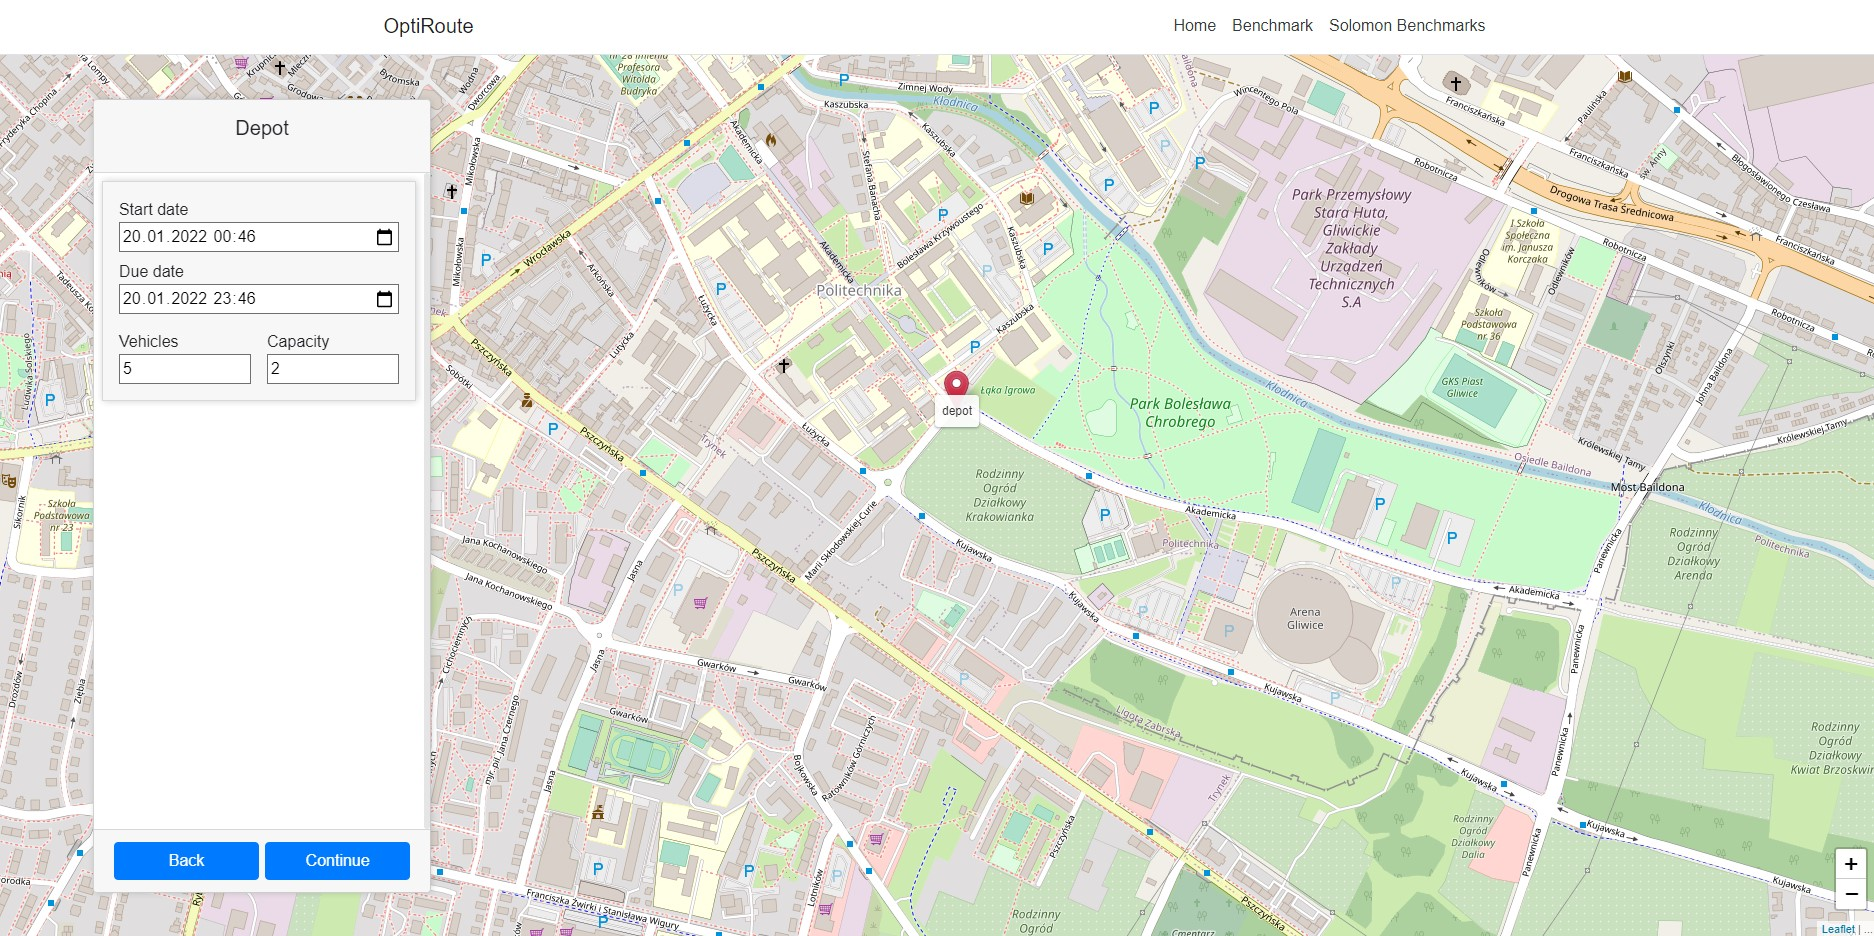
\includegraphics[width=\textwidth]{images/depotScenario1.jpg}
\caption{Usage example 1.1}
\label{fig:depotScenario1}
\end{figure}

\begin{figure}[H]
\centering
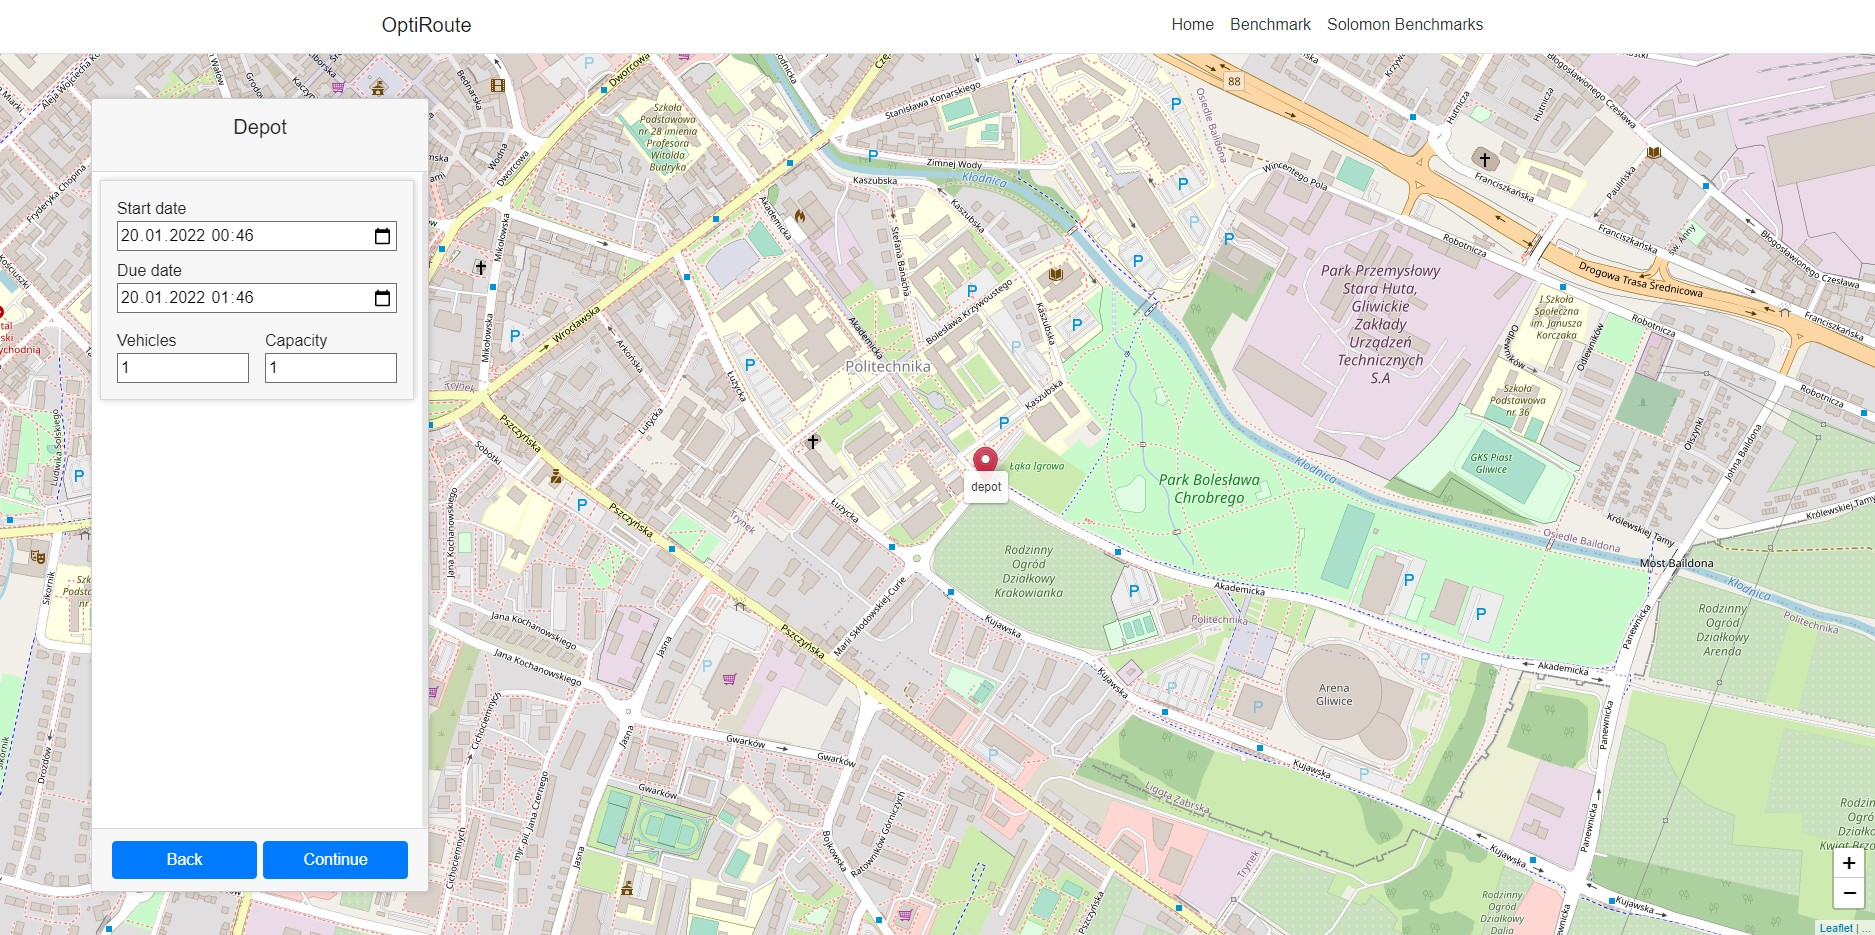
\includegraphics[width=\textwidth]{images/depotScenario2.jpg}
\caption{Usage example 2.1}
\label{fig:depotScenario2}
\end{figure}

\begin{figure}[H]
\centering
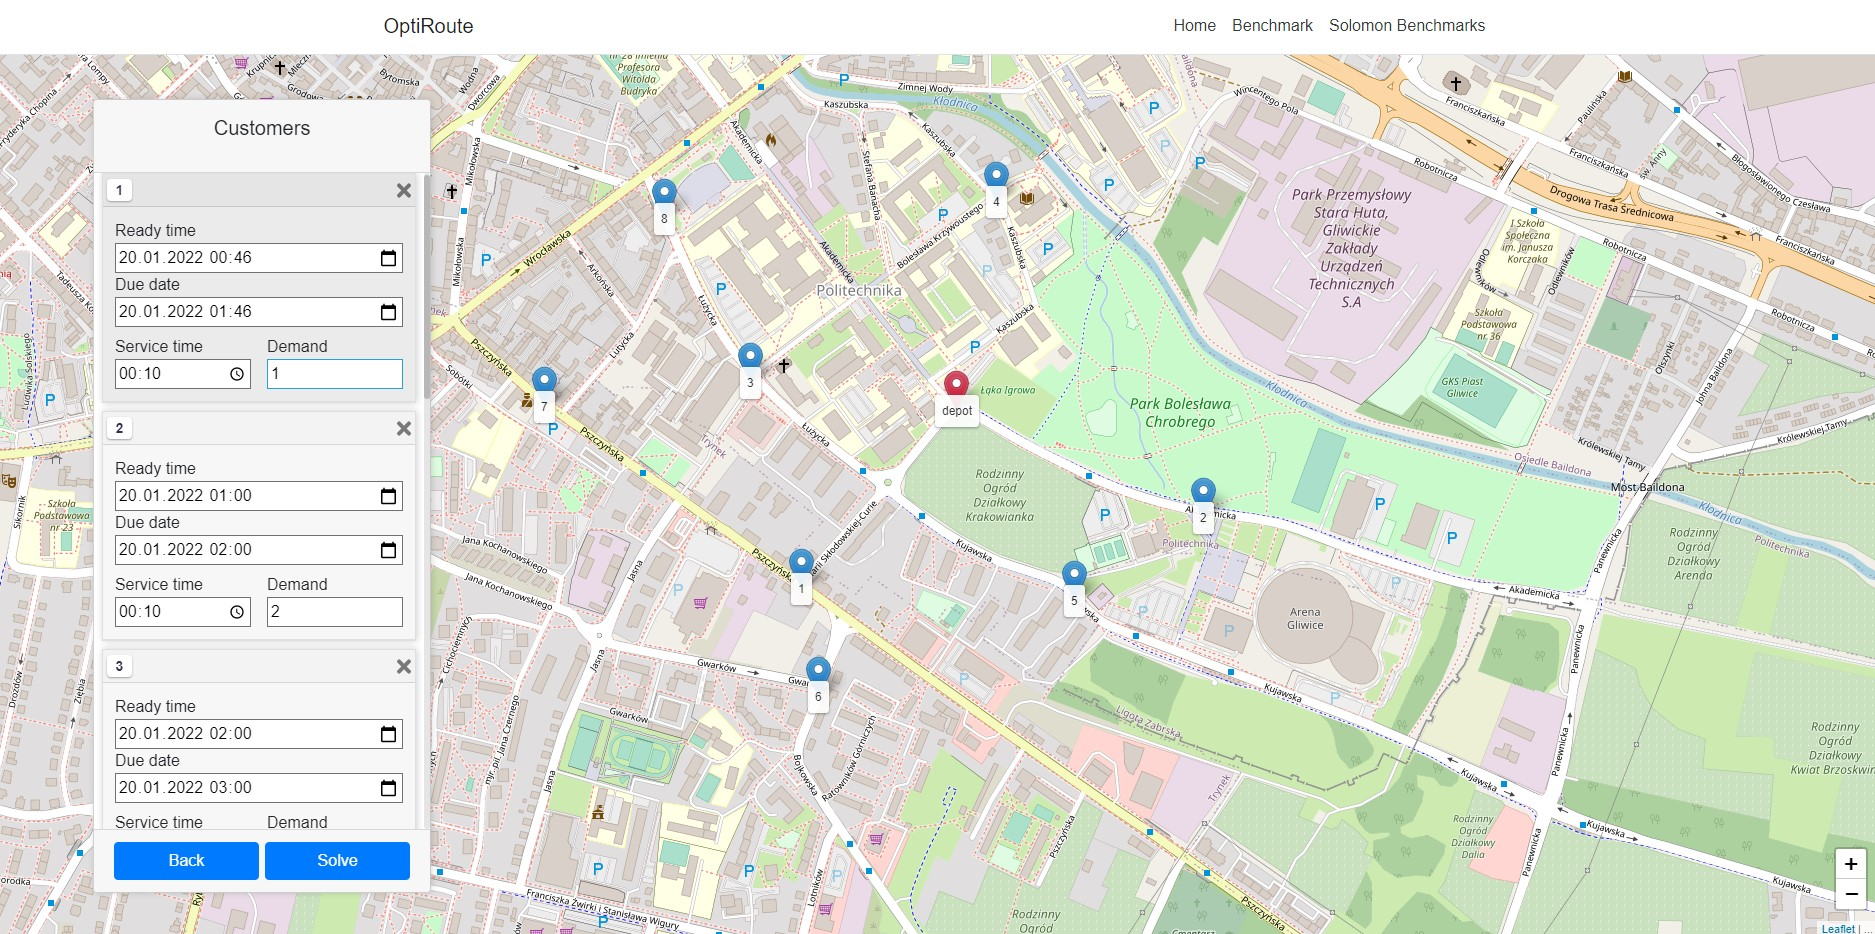
\includegraphics[width=\textwidth]{images/customersScenario1.jpg}
\caption{Usage example 1.2}
\label{fig:customersScenario1}
\end{figure}

\begin{figure}[H]
\centering
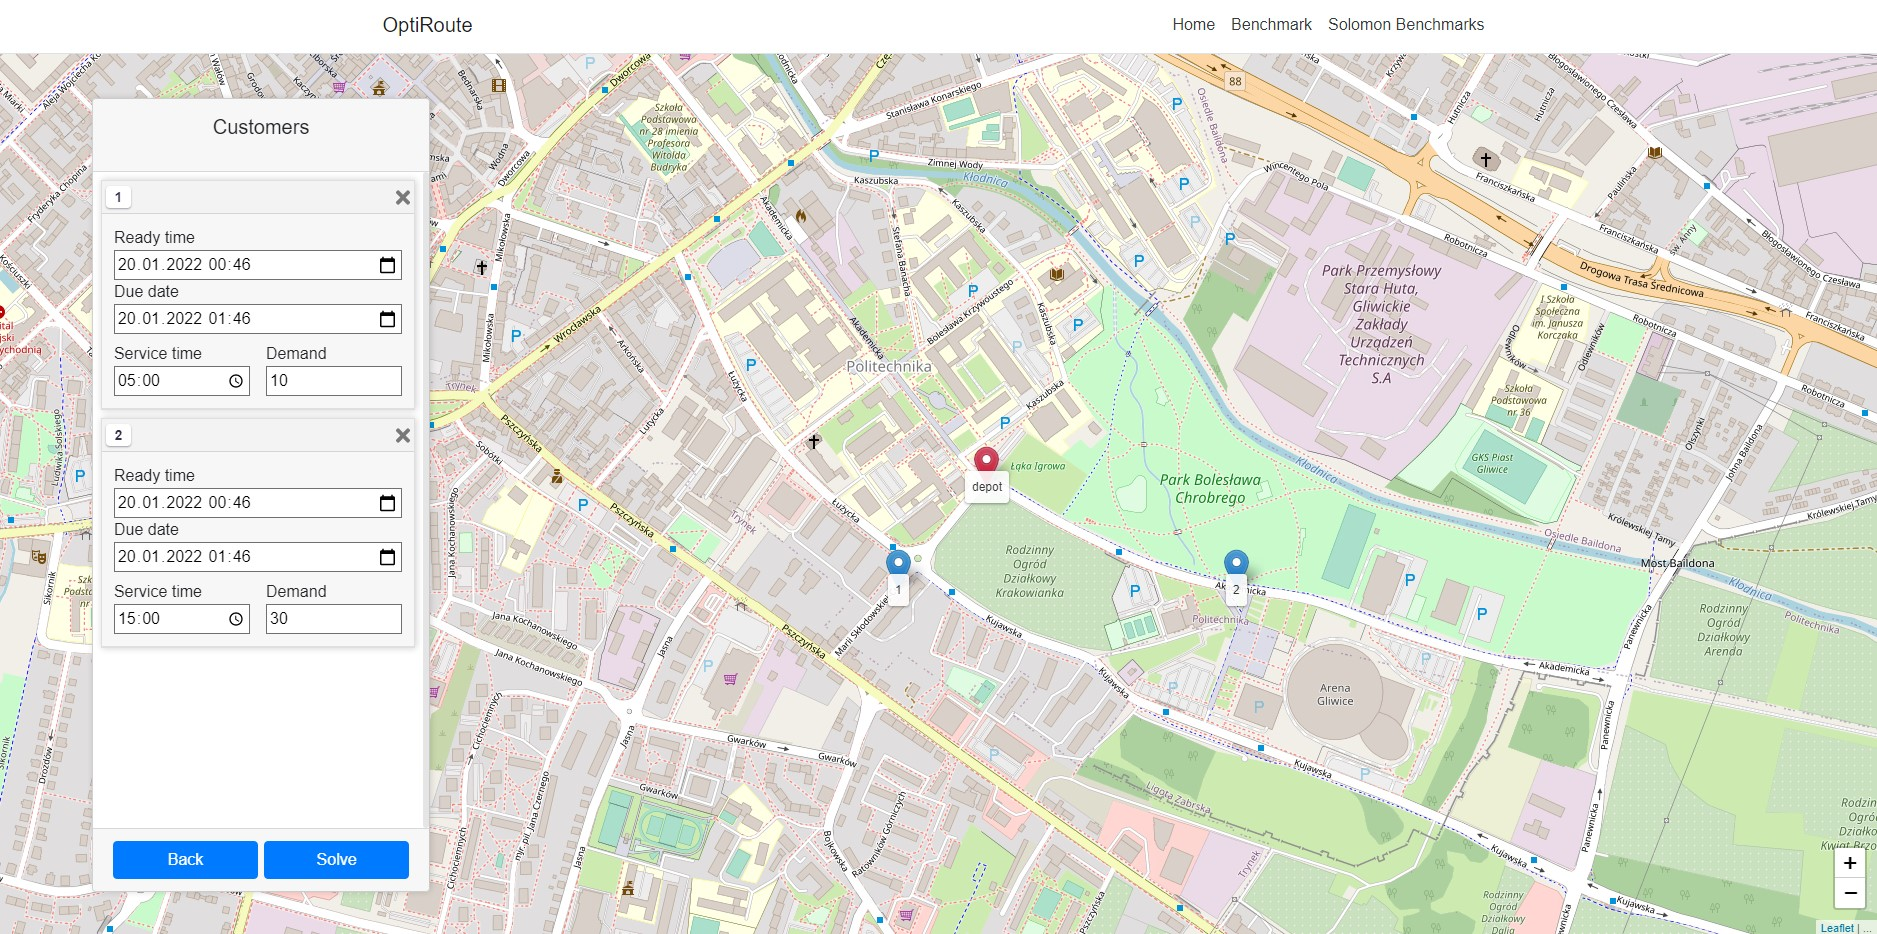
\includegraphics[width=\textwidth]{images/customersScenario2.jpg}
\caption{Usage example 2.2}
\label{fig:customersScenario2}
\end{figure}

\begin{figure}[H]
\centering
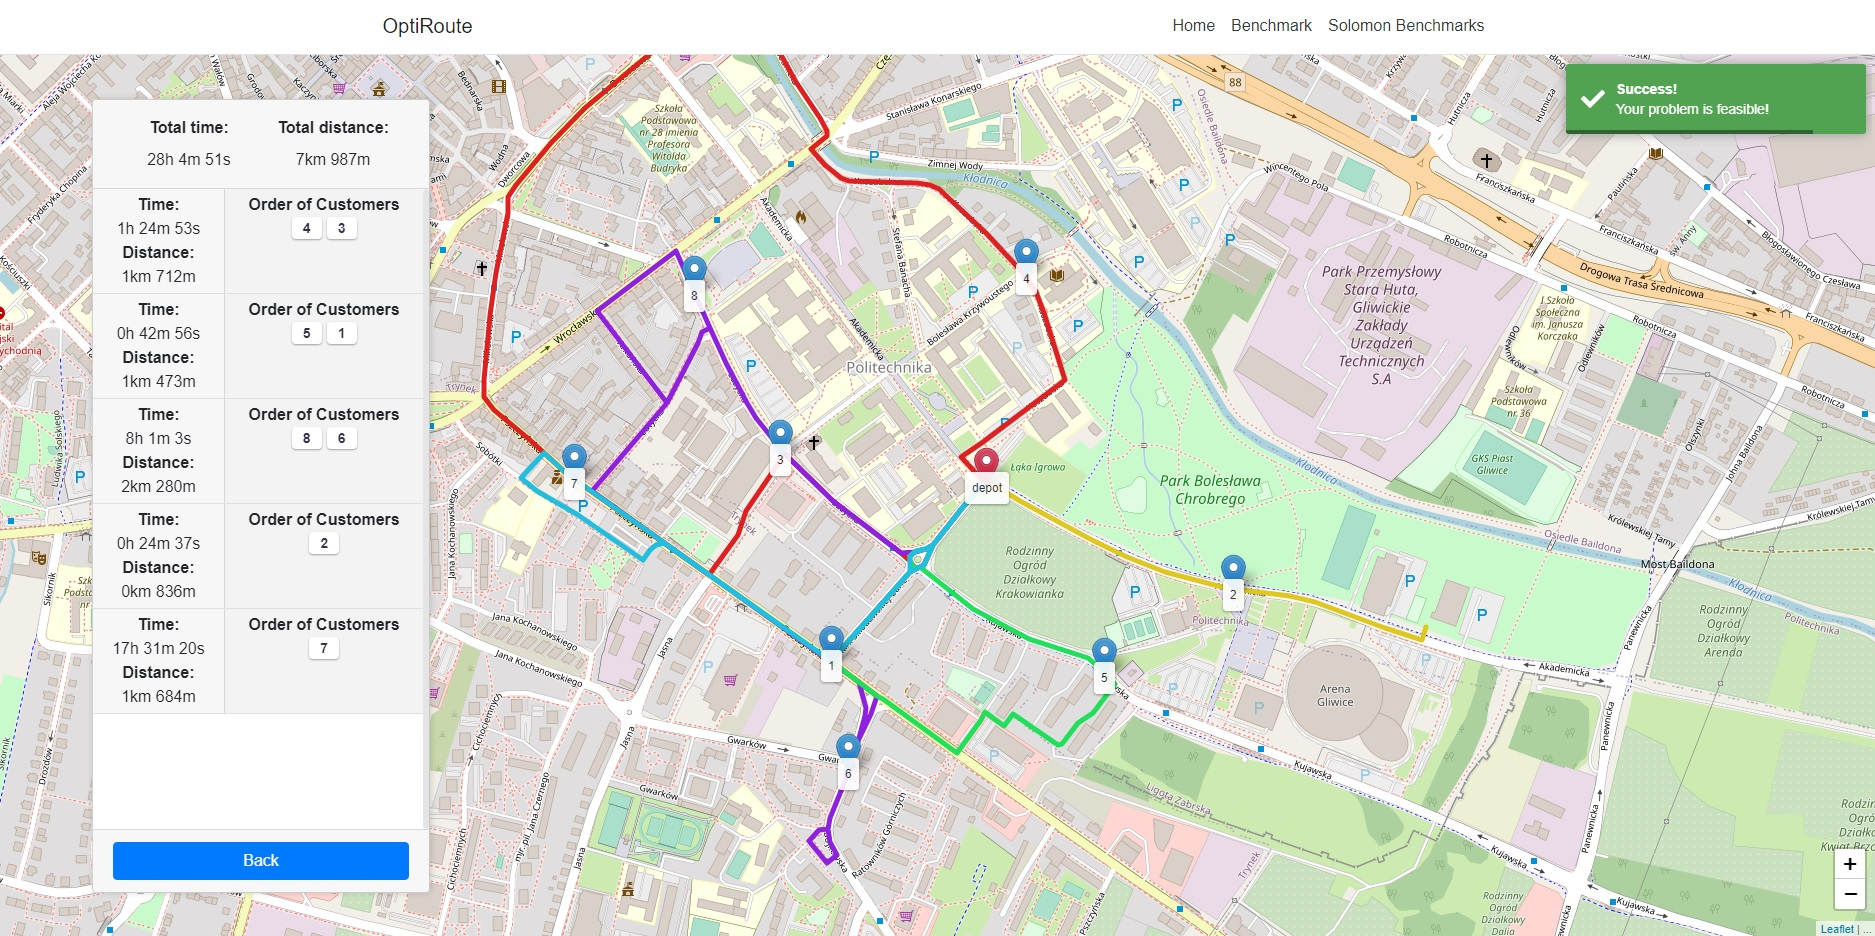
\includegraphics[width=\textwidth]{images/solutionSuccess.jpg}
\caption{Usage example 1.3}
\label{fig:solutionSuccess}
\end{figure}

\begin{figure}[H]
\centering
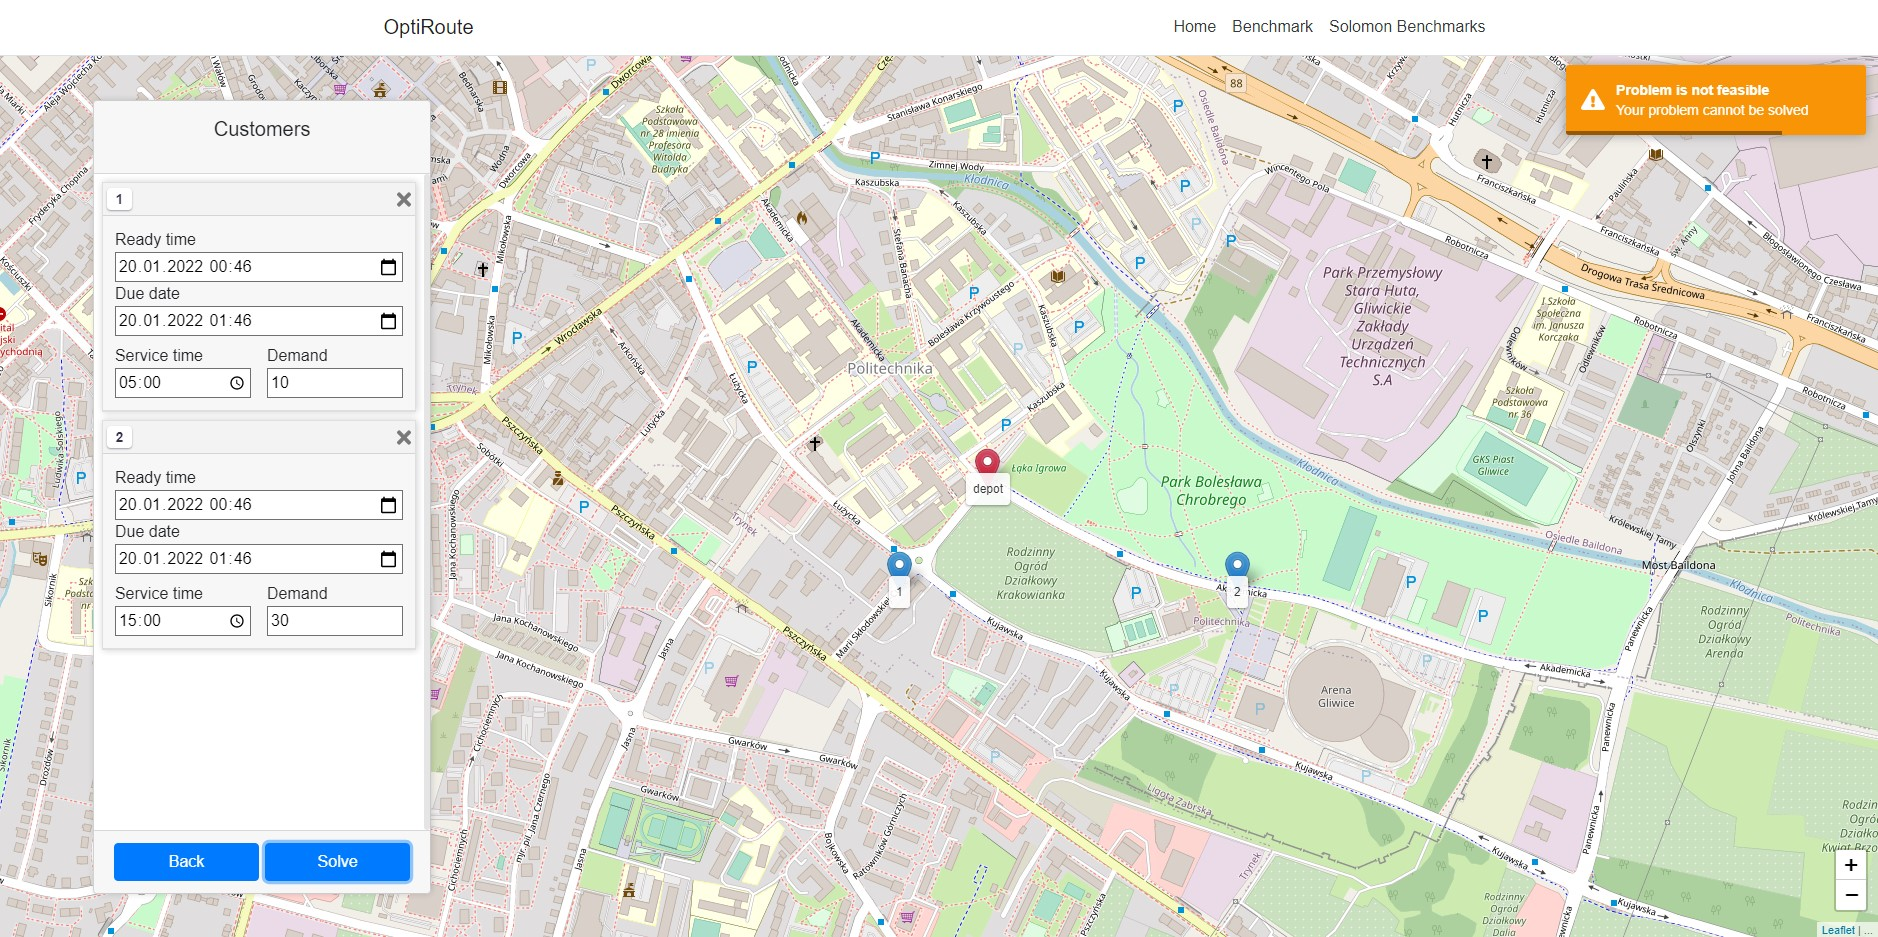
\includegraphics[width=\textwidth]{images/solutionFailed.jpg}
\caption{Usage example 2.3}
\label{fig:solutionFailed}
\end{figure}

\subsection{Benchmark functionality}
User uploads the benchmark file (Figs. \ref{fig:benchmarkFile1} and \ref{fig:benchmarkFile2}) and clicks the "Solve" button. The file is then sent to the backend server and processed by the algorithm. If the problem is solvable a corresponding message appears, details of the solution are displayed and a button to visualize the result (Fig. \ref{fig:benchmarkSuccess}). If the problem cannot be solved an appropriate message is displayed (Fig. \ref{fig:benchmarkFailed}).

\begin{figure}[H]
\centering
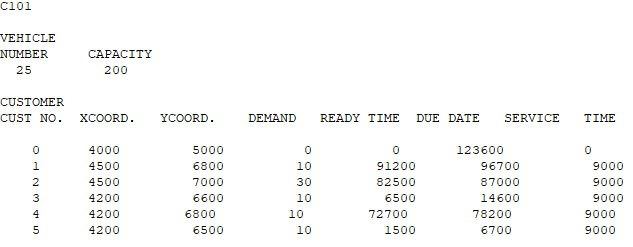
\includegraphics[scale=0.7]{images/benchmarkFile1.jpg}
\caption{Usage example 3.1}
\label{fig:benchmarkFile1}
\end{figure}

\begin{figure}[H]
\centering
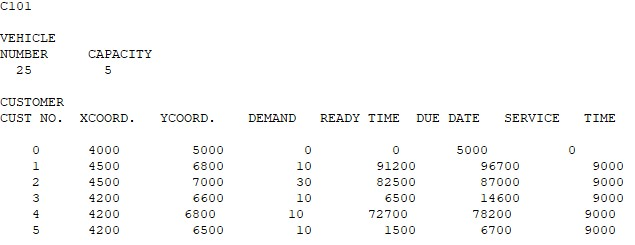
\includegraphics[scale=0.7]{images/benchmarkFile2.jpg}
\caption{Usage example 4.1}
\label{fig:benchmarkFile2}
\end{figure}

\begin{figure}[H]
\centering
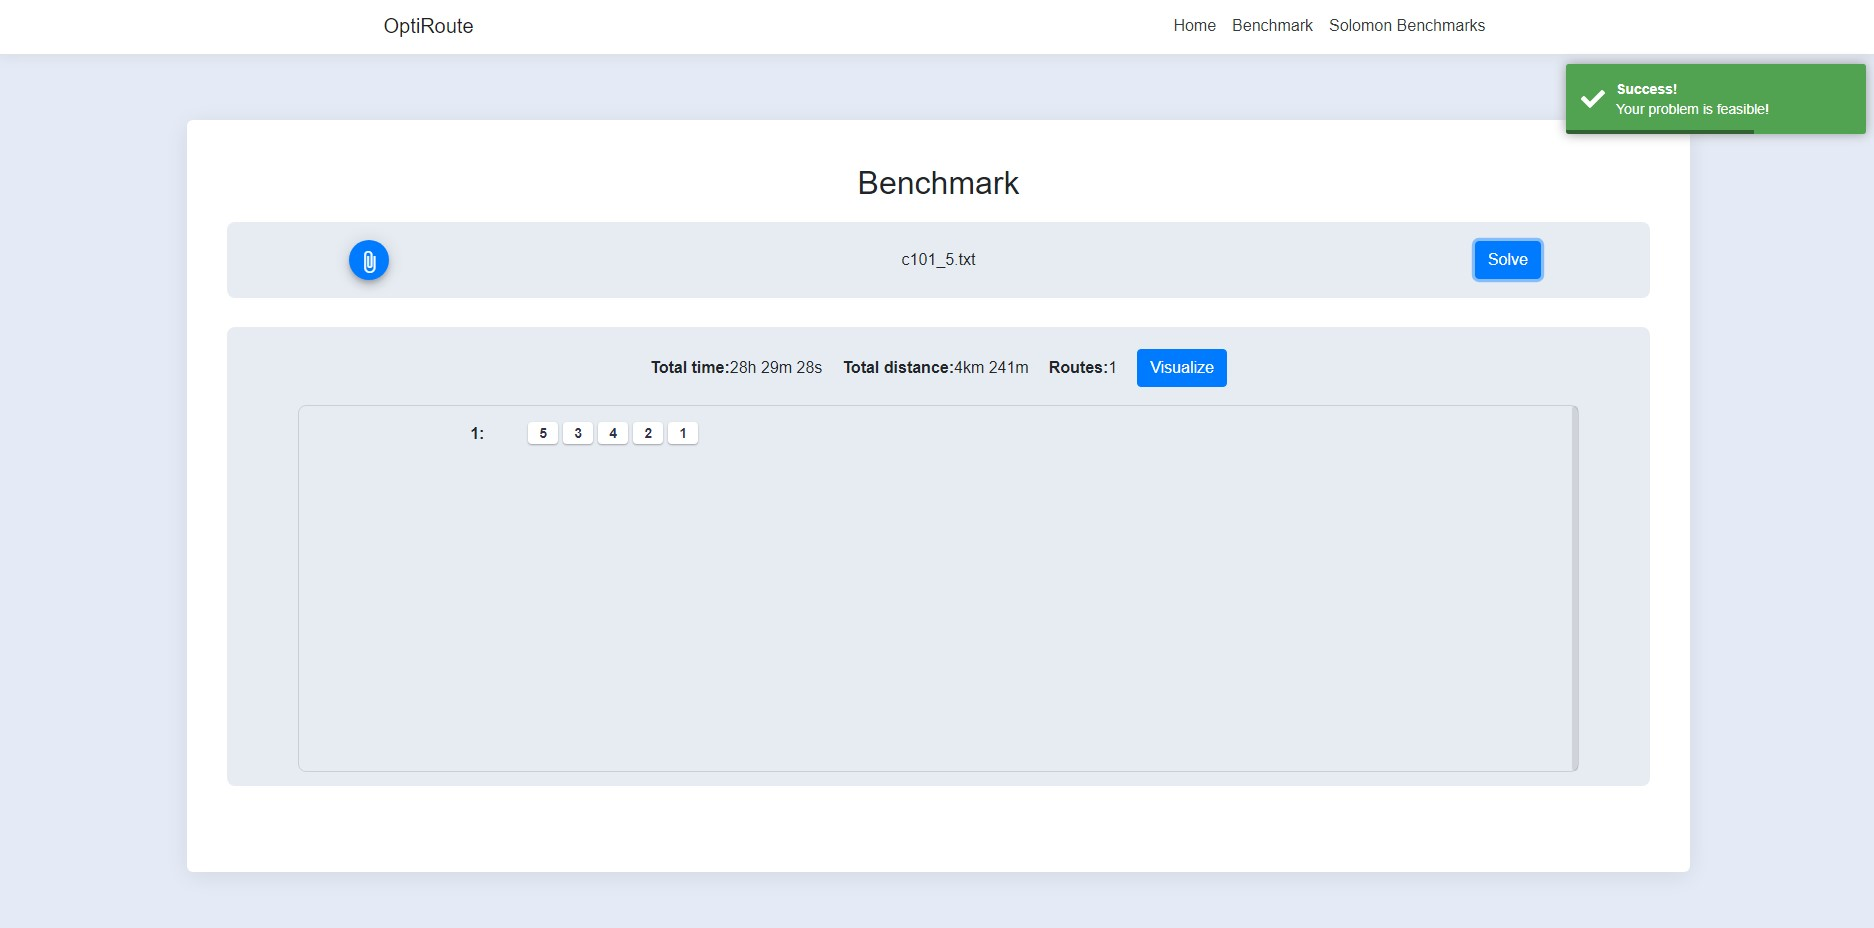
\includegraphics[width=\textwidth]{images/benchmarkSuccess.jpg}
\caption{Usage example 3.2}
\label{fig:benchmarkSuccess}
\end{figure}

\begin{figure}[H]
\centering
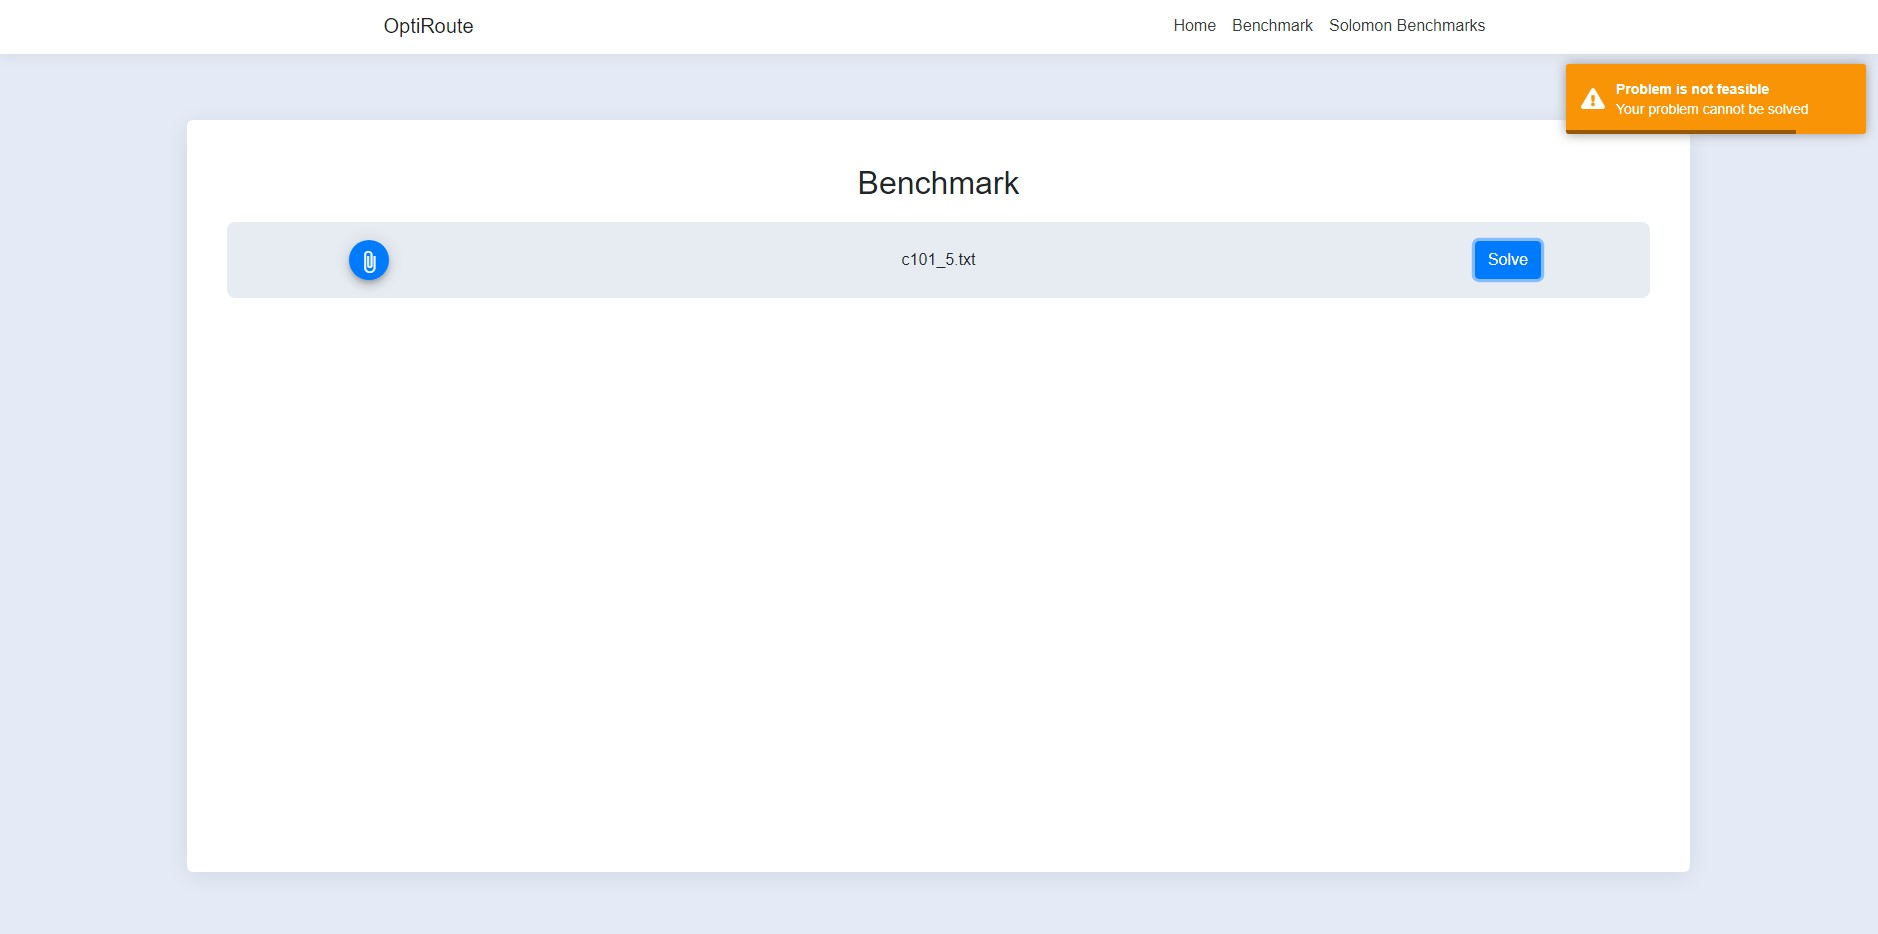
\includegraphics[width=\textwidth]{images/benchmarkFailed.jpg}
\caption{Usage example 4.2}
\label{fig:benchmarkFailed}
\end{figure}


\chapter{Internal specification}

\section{System architecture}
The application implements a client-server architecture with containerized components. The overview of the architecture is presented in Fig. \ref{fig:architectureOverview}. Each component of the system is described in detail later in this chapter.

\begin{figure}
\centering
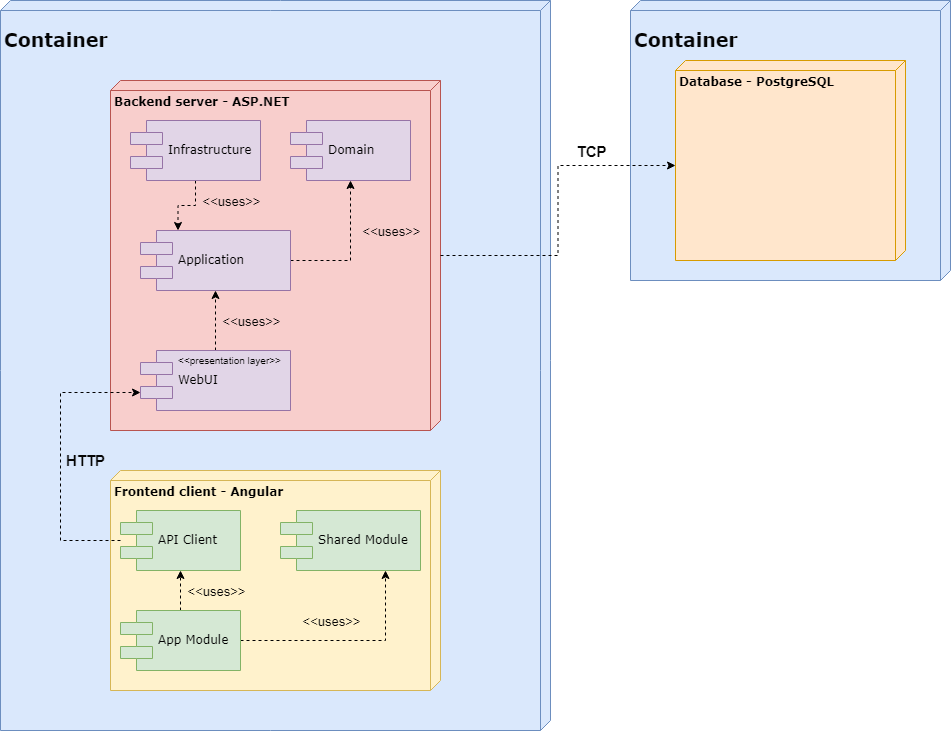
\includegraphics[width=\textwidth]{images/Architecture.drawio.png}
\caption{Architecture overview}
\label{fig:architectureOverview}
\end{figure}

\subsection{Design patterns}
The system was implemented with the use of the three main design patterns: the clean architecture, the command and query responsibility segregation (CQRS) and the mediator pattern. All patterns were used in the backend part of the application.

\subsubsection{Clean architecture}
The backend server is designed according to the clean architecture pattern. The main goal of this architecture is to make the application logic and domain independent from any framework. This approach allows to change any external dependencies e.g. database, web framework or UI while keeping the code of the project core intact. Thanks to the possibility of exchanging external dependencies, the application core can be easily reused in other systems. Moreover, such a system is easily testable, business rules can be tested without any external dependencies.  
The main benefits of this architecture can be outlined as follows \cite{bib:cleanArchitecture}:
\begin{itemize}
\item The system is independent of frameworks - the system can use libraries and frameworks as tools, rather than relying on them and adapting fully to them.
\item Testable - the core of the application can be tested without the external dependencies.
\item Independent of UI - the system may use, for example, a web-based or console UI, but any change to this can be made easily without changing the rest of the system code
\item Independent of database - any database management system can be used, and changing such a system does not affect the core of the application
\end{itemize}
This architecture was chosen to design a system that is modern, scalable and easily expandable.
The structure of the architecture is visible in Fig. \ref{fig:cleanArchitecture}.

\begin{figure}
\centering
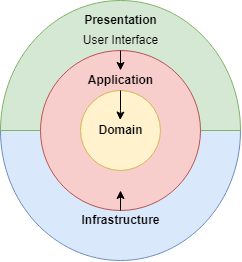
\includegraphics[scale=1]{images/cleanArchitecture.drawio.png}
\caption{Clean architecture}
\label{fig:cleanArchitecture}
\end{figure}

\subsubsection{CQRS}
The command and query responsibility segregation pattern focuses mainly on the separation of data read and write operations. This pattern separates how data is read and written into two models:  
\begin{itemize}
\item Queries - responsible for reading data.
\item Commands - responsible for writing (updating) the data.
\end{itemize}

Furthermore, the pattern abstracts communication between layers and, using the mediator pattern, allows command/query parameters to be separated from their handlers. This approach simplifies the code as a result of reducing the amount of boilerplate code, but most importantly it creates an execution pipeline that allows error handling, logging or validation functionality to be injected \cite{bib:CQRS}. 
\paragraph{}
The benefits of using CQRS pattern
\cite{bib:CQRS}: 
\begin{itemize}
\item Scalability - read operations can be scaled independently of write operations
\item Performance - separate reads and writes can be optimised independently of each other
\item Security - separation ensures that the right class will perform the task
\item Easy to maintain - when the number of available operations is large, each operation is stored in its own source file and is easy to find
\end{itemize}

\subsubsection{Mediator}
A mediator defines an object that encapsulates how a set of objects interact. Instead of communicating directly with each other, objects communicate through a special object called a mediator. The mediator centralises communication between objects, making them dependent only on the mediator, rather than on each object they wish to communicate with \cite{bib:mediator}.

The main benefits of using the mediator design pattern: 
\begin{itemize}
\item Reduces the number of connections between classes
\item Allows easier reuse of individual components
\item The code is easier to maintain
\end{itemize}

The mediator pattern in combination with CQRS provides a set of powerful features and was therefore used in the project \cite{bib:mediatorCQRS}.

\section{Backend server}

\subsection{Used libraries}

\subsubsection{Entity Framework}
Entity Framework is an open-source object-relational mapping (ORM) framework supported by Microsoft. It allows the developer to work with POCO (Plain Old CLR Object) entities without focusing on the underlying database. Entity Framework takes care of creating database connections and executing commands. It also automatically parses the results of queries to the application entities. Another feature of this framework is the ability to track changes to an object and persist those changes to the database. 

Entity Framework introduces the \lstinline|Context| class, which implements the Unit Of Work and Repository patterns. The context class represents a database session and allows various operations to be performed on it. The context class contains \lstinline|DbSet| properties for each of the tables mapped to the application entities. \lstinline|DbSet| is an implementation of the repository pattern. 

Part of the \lstinline|ApplicationDbContext| class used in the project is shown in Fig. \ref{fig:context}.
     
\begin{figure}
\centering
\begin{lstlisting}
        public class ApplicationDbContext : DbContext, IApplicationDbContext
    {
        private readonly IDateTime _dateTime;

        public ApplicationDbContext(
            DbContextOptions options,
            IDateTime dateTime) : base(options)
        {
            _dateTime = dateTime;
        }
        public DbSet<BenchmarkResult> BenchmarkResults { get; set; }
        public DbSet<BenchmarkInstance> BenchmarkInstances { get; set; }
        public DbSet<Route> Routes { get; set; }
        public DbSet<Customer> Customers { get; set; }
        public DbSet<Depot> Depots { get; set; }
        public DbSet<Solution> Solutions { get; set; }
\end{lstlisting}
\caption{Part of the \lstinline|ApplicationDbContext| class.}
\label{fig:context}
\end{figure}

\subsubsection{MediatR}
MediatR is an open-source library that is a simple implementation of the mediator pattern. The library allows in-process messaging without any dependencies. It separates requests from handlers, allowing the principle of single responsibility to be maintained in the code.
MediatR also offers other functionality, such as sending notifications or injecting middlewares for requests called pipeline behaviours.
The main benefits from using the MediatR library: 
\begin{itemize}
\item Less coupled code.
\item Cleaner code because of the requests and handlers separation.
\item Pipeline behaviours that allow data to be processed (e.g. logging) before or after a request is handled.
\end{itemize}

Exemplary request and handler classes used in the project are shown in Fig \ref{fig:mediatR}.

\begin{figure}
\centering
\begin{lstlisting}
    public class GetBestSolutionByBenchmarkResultIdQuery : IRequest<SolutionDto>
    {
        public int BenchmarkResultId { get; set; }
    }

    public class GetBestSolutionByBenchmarkResultIdQueryHandler : IRequestHandler<GetBestSolutionByBenchmarkResultIdQuery, SolutionDto>
    {
        private readonly IApplicationDbContext _context;
        private readonly IMapper _mapper;

        public GetBestSolutionByBenchmarkResultIdQueryHandler(IApplicationDbContext context, IMapper mapper)
        {
            _context = context;
            _mapper = mapper;
        }

        public async Task<SolutionDto> Handle(GetBestSolutionByBenchmarkResultIdQuery request, CancellationToken cancellationToken)
        {
            var result = await _context.Solutions
                .Include(x => x.Depot)
                .Include(x => x.Routes)
                .ThenInclude(x => x.Customers)
                .Include(x => x.BestBenchmarkResult)
                .FirstOrDefaultAsync(x => x.BestBenchmarkResult.DbId == request.BenchmarkResultId);

            return _mapper.Map<SolutionDto>(result);
        }
    }
\end{lstlisting}
\caption{Exemplary request and handler classes.}
\label{fig:mediatR}
\end{figure}


\subsubsection{FluentValidation}
FluentValidation is a library for building strongly typed validation rules. One of the most important features of fluent validation is the separation of validation logic from model and business logic. Each model that should be validated must have its own validator class with validation rules defined inside it. 

The main advantages of using FluentValidation:
\begin{itemize}
\item Easy to work with.
\item Separation of validation rules and models.
\item Clear syntax for validation rules.
\item Speed of execution, allows you to increase the efficiency of the application.
\item Easy to unit test.
\end{itemize}

Sample validator class is shown in Fig. \ref{fig:validator}

\begin{figure}
\centering
\begin{lstlisting}
 public class DepotDtoValidator : AbstractValidator<DepotDto>
    {
        public DepotDtoValidator()
        {
            CascadeMode = CascadeMode.StopOnFirstFailure;

            RuleFor(v => v.Id)
                .NotNull()
                .GreaterThanOrEqualTo(0);

            RuleFor(v => v.X)
               .NotNull()
               .GreaterThanOrEqualTo(0);

            RuleFor(v => v.Y)
               .NotNull()
               .GreaterThanOrEqualTo(0);

            RuleFor(v => v.DueDate)
                .NotEmpty();
        }
    }
\end{lstlisting}
\caption{Validator class for \lstinline|DepotDto| type.}
\label{fig:validator}
\end{figure}

\subsubsection{AutoMapper}
AutoMapper is an object-to-object mapping library. The mapping is performed by transforming an input object of one type to an output object of another type. Mappings between types are fully configurable and allow the programmer to perform complex transformations between types. 
The library simplifies the object mapping process and separates the mapping configurations from the objects, which helps to maintain clean code. Furthermore, another advantage of the library is that it is fully testable.
An example of type mapping configuration is shown in Fig. \ref{fig:autoMapper}.

\begin{figure}
\centering
\begin{lstlisting}
profile.CreateMap<Route, RouteDto>()
                .ForMember(dest => dest.TotalTime, opt => opt.MapFrom(src => src.Vehicle.CurrentTime))
                .ForMember(dest => dest.TotalLoad, opt => opt.MapFrom(src => src.Vehicle.CurrentLoad))
                .ForMember(dest => dest.TotalDistance, opt => opt.MapFrom(src => src.TotalDistance));
\end{lstlisting}
\caption{Configuration of mapping from \lstinline|Route| type to \lstinline|RouteDto| type.}
\label{fig:autoMapper}
\end{figure}

\subsubsection{NSwag}
NSwag provides tools to generate OpenAPI specifications from within ASP.NET Web API controllers. Furthermore, NSwag can generate the typescript API client, reducing the amount of work required to integrate a frontend application with a backend server. The Swagger UI visual documentation (Fig. \ref{fig:swaggerEndpoint}) is also generated by NSwag allowing the developer to test and interact with the API without manually writing implementation logic.  

NSwag was used in the project to speed up the process of integrating the client application with the server and to provide a visual tool to interact and test the API in a convenient way.

\begin{figure} [H]
\centering
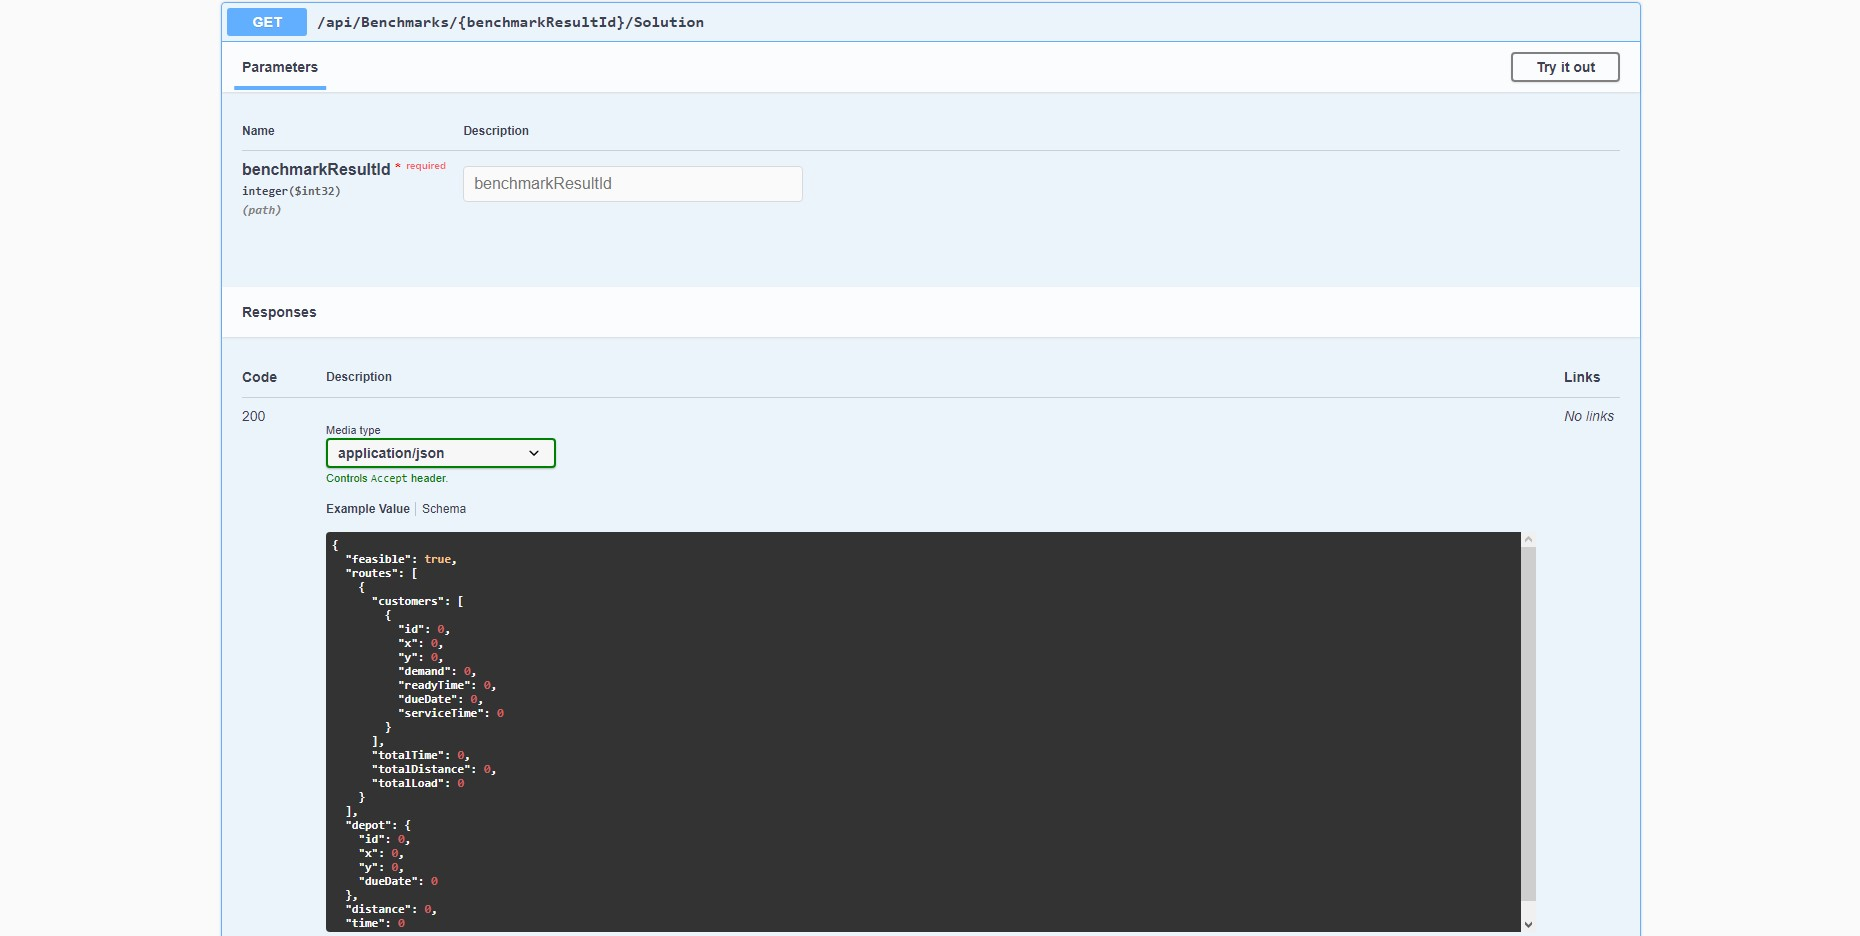
\includegraphics[width=\textwidth]{images/swaggerUI.jpg}
\caption{Swagger UI endpoint.}
\label{fig:swaggerEndpoint}
\end{figure}

\subsubsection{NUnit}
NUnit is an open-source unit testing framework for the .NET platform. The framework is easy to work with and provides various tools to create good and reliable unit tests for applications.

\subsection{Domain}

The project domain layer contains all the entities and their logic specific to the domain layer. The business domain of the application is modelled inside this layer. The term domain layer comes from the Domain Driven Design (DDD) approach to structuring software. 

There are two main approaches when it comes to implementing domain entities:
\begin{itemize}
    \item Anemic model - separates the logic from models. The logic is placed in separated classes (services, helpers etc.).
    \item Rich model - each model has its own behavioural logic encapsulated inside an entity.  For example, the \lstinline|Cart| entity will contain an \lstinline|AddProductToCart| method inside the class.
\end{itemize}

The rich domain model approach was chosen for the project because it preserves one of the most important aspects of object-oriented programming (OOP), which is encapsulation. With a rich domain model, the code is cleaner and more secure (because sensitive data is only stored and modified inside the model) than with an anemic model. Furthermore, the domain is easier to maintain, and a rich model prevents the application from creating invalid domain objects. The rich domain entities can be easily unit tested without the need to call any external services to apply business logic to them.

The domain project contains all the entities that are used in the application: 
\begin{itemize}
    \item \lstinline|BenchmarkInstance| - contains information about the instance of the Solomon benchmark problem.
    \item \lstinline|BenchmarkResult| - stores the \lstinline|BenchmarkInstance| and the \lstinline|Solution| generated by the application and the best known \lstinline|Solution|.
    \item \lstinline|Customer| - represents the customer in the CVRPTW. Includes methods for calculating the distance and duration of a travel to another \lstinline|Customer| or \lstinline|Depot|.
    \item \lstinline|Depot| - represents the depot.
    \item \lstinline|Problem| - defines the CVRPTW. It contains the details of the problem, the \lstinline|Depot|, the \lstinline|Customer| list and tables of distances and travel times between each location in the problem.
    \item \lstinline|Route| -  represents a route. It contains methods for i.a. adding or removing a \lstinline|Customer| from the route, validating time and capacity limits (Fig. \ref{fig:routeMethod}).
    \item \lstinline|Solution| - the solution produced by the algorithm.
    \item \lstinline|Vehicle| -  represents the vehicle in the CVRPTW.   
\end{itemize}

The project domain layer does not depend on any external library and can be reused in other projects as the core of the system.

\begin{figure}
\centering
\begin{lstlisting}
public class Route
    {
            public void AddCustomer(Customer customer)
        {
            if (Customers.Count > 0)
            {
                CustomersDistance += this.Customers.Last().CalculateDistanceBetween(this.Distances, customer);
                CustomersTime += this.Customers.Last().CalculateTimeBetween(this.Durations, customer);
            }
            this.Customers.Add(customer);

            if (TimeFromDepot + CustomersTime + WaitingTime < customer.ReadyTime)
            {
                double waitingTime = customer.ReadyTime - (TimeFromDepot + CustomersTime + WaitingTime);
                this._waitingTime += waitingTime;
                this._waitingTimeDictionary.Add(customer.Id, waitingTime);
            }

            CustomersTime += customer.ServiceTime;

            this.Vehicle.CurrentLoad += customer.Demand;
            this.Vehicle.CurrentTime = this.TotalTime;
        }
                public bool IsFeasible()
        {
            if (CheckCapacityConstraints())
                return CheckTimeConstraints();

            return false;
        }
\end{lstlisting}
\caption{Part of the Route entity class.}
\label{fig:routeMethod}
\end{figure}




\subsection{Application}

\subsection{Infrastructure}

\subsection{Presentation}

\section{Frontend client}

\subsection{Used libraries}

\subsection{App module}

\subsection{Shared module}

\subsection{API client}

\begin{itemize}
\item concept of the system
\item system architecture
\item description of data structures (and data bases)
\item components, modules, libraries, resume of important classes (if used)
\item resume of important algorithms (if used)
\item details of implementation of selected parts
\item applied design patterns
\item UML diagrams
\end{itemize}


Use special environment for inline code, eg \lstinline|descriptor| or \lstinline|descriptor_gaussian|. 
Longer parts of code put in the figure environment, eg. code in Fig. \ref{fig:pseudokod}. Very long listings–move to an appendix.

% \begin{figure}
% \centering
% \begin{lstlisting}
% class descriptor_gaussian : virtual public descriptor
% {
%   protected:
%       /** core of the gaussian fuzzy set */
%       double _mean;
%       /** fuzzyfication of the gaussian fuzzy set */
%       double _stddev;
      
%   public:
%       /** @param mean core of the set
%           @param stddev standard deviation */
%       descriptor_gaussian (double mean, double stddev);
%       descriptor_gaussian (const descriptor_gaussian & w);
%       virtual ~descriptor_gaussian();
%       virtual descriptor * clone () const;
      
%       /** The method elaborates membership to the gaussian fuzzy set. */
%       virtual double getMembership (double x) const;
     
% };
% \end{lstlisting}
% \caption{The \lstinline|descriptor_gaussian| class.}
% \label{fig:pseudokod}
% \end{figure}


\chapter{Verification and validation}
\section{Testing and validation}
During the development process, different parts of the application were tested in different ways. The most difficult task was to test the algorithm and make sure that it gave correct solutions to the given problems. 
\subsection{Algorithm and backend}
The correctness of the solutions was achieved by combining several testing and validation techniques.

\subsubsection{Visualization tool}
At the beginning of the application development process, when only the algorithmic part was under development, a simple visualisation tool was created. The purpose of this tool was to visually check that the resulting solutions were created in a meaningful and in some sense optimal way. The visualisation tool was necessary in the early stages of the application development because of the interpretability of the results generated by the algorithm. Detecting irregularities in the operation of the algorithm by reading the produced routes in text form is, for larger problems, an almost impossible task. The person validating the solution would have to remember, for example, the coordinates of 50 clients and the time windows of each of them and check the routes considering each constraint of the problem. Thanks to the visualisation tool, the process of initial validation at that stage of development was significantly facilitated.

The tool was also useful after the heuristic part of the algorithm was completed. It was easy to observe the improvement in the solutions (Fig. \ref{fig:visualizationTestExample}).

\begin{figure}[H]
\centering
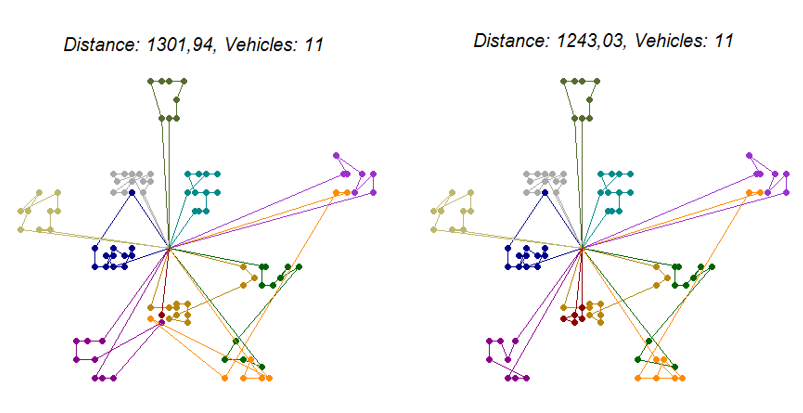
\includegraphics[width=\textwidth]{images/visualizationTestExample.png}
\caption{Initial and improved solutions visualized by the tool}
\label{fig:visualizationTestExample}
\end{figure}

\subsubsection{Solomon Benchmarks}
Solomon benchmark instances were used not only to evaluate the performance of the algorithm, but also to test and validate its operation. This was achieved by comparing the routes produced by the algorithm with the ones from the best known solutions. After comparison, it was observed that in most cases the routes were similar and differed by only a few customers. The difference in customers was reflected in the total distance and number of vehicles used in the solutions developed by the algorithm.

\subsubsection{Unit tests}
Unit tests played a key role in eliminating errors in the algorithmic part of the application. Each domain object has corresponding unit tests, and every functionality within each object is fully covered by unit tests. Unit tests have facilitated the software development process by allowing to check that all functionality works correctly after each change. Furthermore, during the development of the unit tests, it was discovered that the algorithm calculated the total time of each route without taking into account the waiting time before the time window. The error was quickly fixed, which would have been much more difficult and time-consuming without the help of unit tests.

An exemplary part of unit tests class for the \lstinline|Route| object is shown in Fig. \ref{fig:routeUnitTests}.
An exemplary run of domain unit tests is visible in Fig \ref{fig:unitTestsRun}.

\begin{figure}
\centering
\begin{lstlisting}
   public class RouteTests
{
                [Test]
        [TestCaseSource(typeof(EntityHelper), nameof(EntityHelper.PrepareCustomerCases))]
        public void ShouldChangeLoadOfTheVehicle(List<Customer> customers)
        {
            Route route = EntityHelper.GetRouteCase(0, 5, 100);


            foreach (var customer in customers)
            {
                customer.CalculateDepotTimesAndDistances(route.Distances, route.Durations);
                route.AddCustomer(customer);
            }

            route.Vehicle.CurrentLoad.Should().Be(customers.Sum(x => x.Demand));
        }

        [Test]
        [TestCaseSource(typeof(EntityHelper), nameof(EntityHelper.PrepareCustomerCases))]
        public void ShouldNotChangeLoadOfTheVehicle(List<Customer> customers)
        {
            Route route = EntityHelper.GetRouteCase(0, 5, 100);


            foreach (var customer in customers)
            {
                customer.CalculateDepotTimesAndDistances(route.Distances, route.Durations);
                route.AddCustomer(customer);
                route.DeleteCustomer(customer);
            }

            route.Vehicle.CurrentLoad.Should().Be(0);
        }
}

\end{lstlisting}
\caption{Part of the \lstinline|RouteTests| class.}
\label{fig:routeUnitTests}
\end{figure}

\begin{figure}
\centering
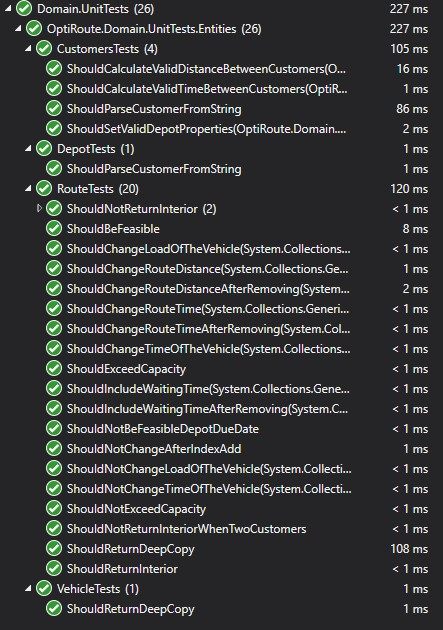
\includegraphics[width=\textwidth]{images/domainTests.jpg}
\caption{Domain unit tests}
\label{fig:unitTestsRun}
\end{figure}

\subsubsection{Manual tests}
The algorithm and the entire backend part of the application were also tested manually. The API was tested using the Swagger UI (Fig. \ref{fig:swagger}). During development, each endpoint was tested by sending various valid and invalid requests, by observing the responses it was possible to determine if the functionality was working correctly or not. 

\begin{figure}
\centering
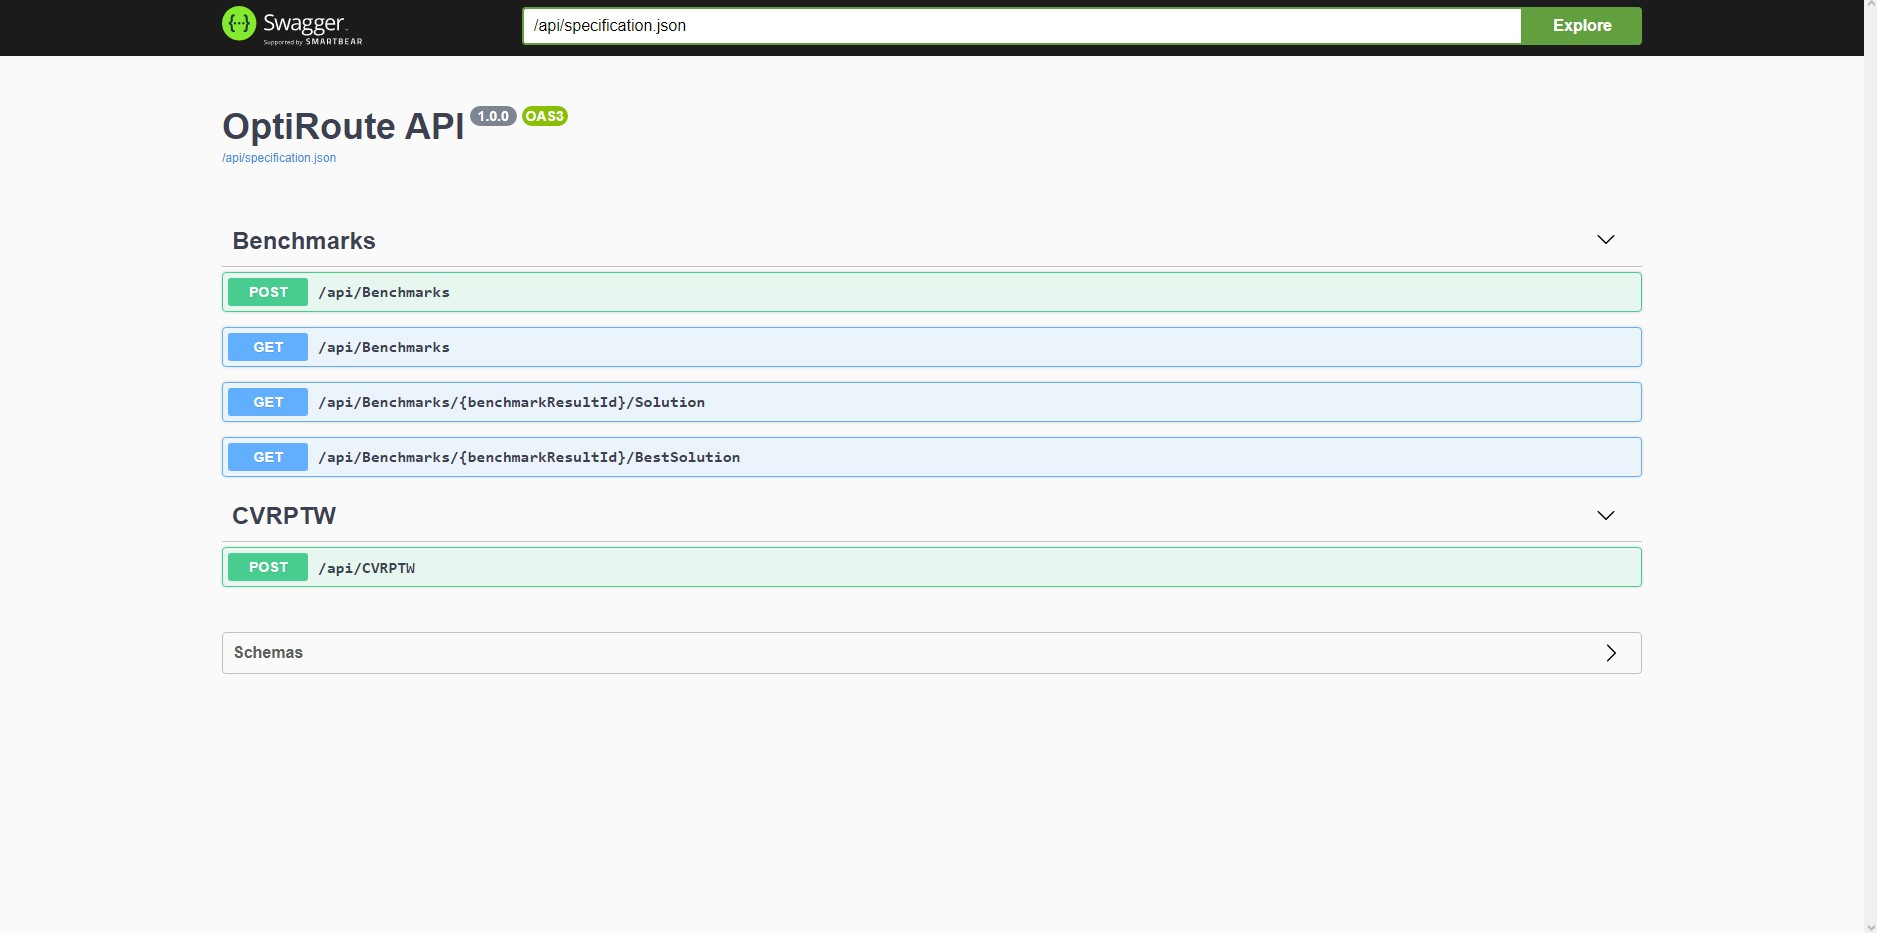
\includegraphics[width=\textwidth]{images/swagger.jpg}
\caption{Swagger UI}
\label{fig:swagger}
\end{figure}


In a further stage of development, the algorithm was tested manually using a frontend client application. Using the frontend client, a number of problems were defined and solved, including a group of relatively small problems of low complexity, which made manual verification easier (small number of clients, vehicles and distances between points). This process made it possible to find and fix small errors and to prove the correctness of the algorithm. The summary times and distances for each route obtained by the algorithm were as expected. 
In addition, each API endpoint used in the frontend client was also manually tested along with the request data validation mechanisms. 

\subsection{Client}
The specifics of creating a front-end application allows the developer to test functionality at every stage of its development, from the visual side to the logic of individual components. The client application was tested on different screen resolutions in order to achieve responsiveness. The request data is also validated on the client side of the application, so it was checked whether the information about the incorrect data is displayed correctly. In addition, toast pop-ups were tested to check the readability of messages and the correct implementation of the error handling mechanism. 

\section{Solomon benchmark results}
In order to evaluate the performance of the algorithm, it was tested on all Solomon benchmark instances. A comparison of the best known solutions with the solutions obtained by the algorithm is shown in the tables \ref{tab:solomonPart1} and \ref{tab:solomonPart2} \cite{bib:solomonSintef}.


\begin{table}
\centering
\caption{Solomon benchmark instances C101 - R111}
\label{tab:solomonPart1}
\begin{tabular}{rrrrr}
\toprule
	         &\multicolumn{2}{c}{Thesis} & \multicolumn{2}{c}{Best} \\
	         \cmidrule(r){2-3}\cmidrule(r){4-5}
	Instance &     Distance &  Vehicles & Distance & Vehicles \\
\midrule
 C101 & 878.36 & 10 & 828.94 & 10 \\ 
 C102 & 1326.54 & 11 & 828.94 & 10 \\ 
 C103 & 1617.72 & 11 & 828.06 & 10 \\ 
 C104 & 1219.16 & 11 & 824.78 & 10 \\ 
 C105 & 953.79 & 10 & 828.94 & 10 \\ 
 C106 & 1103.6 & 10 & 828.94 & 10 \\ 
 C107 & 1127.49 & 10 & 828.94 & 10 \\ 
 C108 & 1191.96 & 10 & 828.94 & 10 \\ 
 C109 & 1380.5 & 10 & 828.94 & 10 \\ 
 C201 & 635.21 & 3 & 591.56 & 3 \\ 
 C202 & 1553.27 & 4 & 591.56 & 3 \\ 
 C203 & 1798.73 & 4 & 591.17 & 3 \\ 
 C204 & 1408.45 & 4 & 590.6 & 3 \\ 
 C205 & 903.72 & 4 & 588.88 & 3 \\ 
 C206 & 972.93 & 4 & 588.49 & 3 \\ 
 C207 & 1095.88 & 4 & 588.29 & 3 \\ 
 C208 & 974.34 & 3 & 588.32 & 3 \\ 
 R101 & 2181.6 & 22 & 1650.8 & 19 \\ 
 R102 & 2105.3 & 19 & 1486.12 & 17 \\ 
 R103 & 1851.02 & 17 & 1292.68 & 13 \\ 
 R104 & 1613.99 & 14 & 1007.31 & 9 \\ 
 R105 & 1931.59 & 17 & 1377.11 & 14 \\ 
 R106 & 1710.02 & 15 & 1252.03 & 12 \\ 
 R107 & 1825.93 & 16 & 1104.66 & 10 \\ 
 R108 & 1696.73 & 13 & 960.88 & 9 \\ 
 R109 & 1823.1 & 15 & 1194.73 & 11 \\ 
 R110 & 1864.64 & 14 & 1118.84 & 10 \\ 
 R111 & 1791.79 & 14 & 1096.72 & 10 \\ 

\bottomrule
\end{tabular}
\end{table}  

\begin{table}
\centering
\caption{Solomon benchmark instances R112 - RC208}
\label{tab:solomonPart2}
\begin{tabular}{rrrrr}
\toprule
	         &\multicolumn{2}{c}{Thesis} & \multicolumn{2}{c}{Best} \\
	         \cmidrule(r){2-3}\cmidrule(r){4-5}
	Instance &     Distance &  Vehicles & Distance & Vehicles \\
\midrule
 R112 & 1515.72 & 12 & N/A & N/A \\ 
 R201 & 2137.77 & 5 & 1252.37 & 4 \\ 
 R202 & 1950.89 & 5 & 1191.7 & 3 \\ 
 R203 & 1781.85 & 4 & N/A & N/A \\ 
 R204 & 1627.31 & 4 & 825.52 & 2 \\ 
 R205 & 2037.2 & 4 & 994.43 & 3 \\ 
 R206 & 1867.63 & 4 & 906.14 & 3 \\ 
 R207 & 1915.13 & 3 & N/A & N/A \\ 
 R208 & 1529.16 & 3 & 726.82 & 2 \\ 
 R209 & 1960.98 & 4 & 909.16 & 3 \\ 
 R210 & 1947.06 & 4 & 939.37 & 3 \\ 
 R211 & 1614.42 & 3 & N/A & N/A \\ 
 RC101 & 2192.4 & 17 & 1696.95 & 14 \\ 
 RC102 & 2281.54 & 17 & 1554.75 & 12 \\ 
 RC103 & 1975.79 & 15 & 1261.67 & 11 \\ 
 RC104 & 1772.02 & 13 & 1135.48 & 10 \\ 
 RC105 & 2210.6 & 18 & 1629.44 & 13 \\ 
 RC106 & 1969.33 & 15 & 1424.73 & 11 \\ 
 RC107 & 1828.77 & 14 & N/A & N/A \\ 
 RC108 & 1969.33 & 13 & 1139.82 & 10 \\ 
 RC201 & 2639.03 & 5 & 1406.94 & 4 \\ 
 RC202 & 2382.9 & 4 & N/A & N/A \\ 
 RC203 & 2098.92 & 4 & N/A & N/A \\ 
 RC204 & 1743.92 & 4 & 798.46 & 3 \\ 
 RC205 & 2395.17 & 5 & 1297.65 & 4 \\ 
 RC206 & 1886.68 & 4 & 1146.32 & 3 \\ 
 RC207 & 1942.84 & 4 & 1061.14 & 3 \\ 
 RC208 & 1772.11 & 3 & 828.14 & 3 \\ 
\bottomrule
\end{tabular}
\end{table}  

 

\chapter{Conclusions}
\section{Achieved results}
The primary objective of the work was to design and implement a tool that would simplify the process of defining and solving CVRPTW for the end user. This objective was successfully achieved and a modern and user-friendly web application was implemented. All functional and non-functional requirements that were identified in the early stages of development have been met. The implemented algorithm solves the VRP in a fast way and the results obtained can be considered satisfactory. The containerisation of the project makes it easy to run and deploy, which increases the usability of the application.

\section{Further development}
Although the application has met the requirements and expectations, there is room for improvement. One of the biggest areas with possibilities to extend the system is the VRP itself, there are many variations of the problem that take into account more constraints. In addition, the algorithmic part of the application could be extended to implement other heuristic and meta-heuristic methods that could potentially improve the performance of the algorithm.

The application could also be extended to include users and their management. Users would be able to save a problem, view the history of their previous problems and solutions, or upload their own benchmark files and share them with other users.

A mobile version of the application could also be a significant improvement. A portable version of the application would increase its usability.

There are still opportunities for further enhancements in the testing part of the application. Integration tests or end-to-end tests could be implemented to make the application more reliable and the development process even easier.
The prospects for future development are broad and, thanks to the way the application has been designed, would not require rebuilding the existing code base and the system could be easily extended without much effort.

\section{Encountered difficulties and problems}
The most difficult problem encountered during the development process was adapting the LeafletJS and Leaflet Routing Machine libraries to the needs of the project. There is not much information on the internet about redrawing multiple routes on the map or removing them. In the end, the desired effect was achieved and there was no need to change any of the libraries. 

The process of containerising the application was very time consuming and required extensive research. The most difficult task was to create a correct docker file and to integrate the process of building both the server and client parts of the application.

The algorithmic part of the application was completed without any major problems, but the most difficult part of this stage of development was the correct calculation of time and distance when a client was added or removed from the route. However, thanks to unit testing, this functionality was completed in a reasonably short time.

 

 


%%%%%%%%%%%%%%%%%%%%%%%%%%%%%%%%%%%%%%%%%%
\backmatter
\pagenumbering{Roman}
\stepcounter{PagesWithoutNumbers}
\setcounter{page}{\value{PagesWithoutNumbers}}

\pagestyle{onlyPageNumbers}

%%%%%%%%%%% bibliography %%%%%%%%%%%%
%\bibliographystyle{plain}
%\bibliography{bibliography}

\addcontentsline{toc}{chapter}{Bibliography}
\printbibliography
%%%%%%%%%  appendices %%%%%%%%%%%%%%%%%%% 

\begin{appendices} 


 

\chapter*{Index of abbreviations and symbols}
\addcontentsline{toc}{chapter}{Index of abbreviations and symbols}

\begin{itemize}
\item[VRP] Vehicle Routing Problem
\item[VRPTW] Vehicle Routing Problem with Time Windows
\item[CVRPTW] Capacitated Vehicle Routing Problem with Time Windows
\item[$V$] Set of vertices representing customers and the depot
\item[$A$] Arcs connecting vertices from $V$
\item[$W$] Set of vehicles
\item[$Q$] Capacity of vehicle
\end{itemize}


\chapter*{Listings}
\addcontentsline{toc}{chapter}{Listings}

(Put long listings in the appendix.)

\begin{lstlisting}
partition fcm_possibilistic::doPartition
                             (const dataset & ds)
{
   try
   {
      if (_nClusters < 1)
         throw std::string ("unknown number of clusters");
      if (_nIterations < 1 and _epsilon < 0)
         throw std::string ("You should set a maximal number of iteration or minimal difference -- epsilon.");
      if (_nIterations > 0 and _epsilon > 0)
         throw std::string ("Both number of iterations and minimal epsilon set -- you should set either number of iterations or minimal epsilon.");
   
      auto mX = ds.getMatrix();
      std::size_t nAttr = ds.getNumberOfAttributes();
      std::size_t nX    = ds.getNumberOfData();
      std::vector<std::vector<double>> mV;
      mU = std::vector<std::vector<double>> (_nClusters);
      for (auto & u : mU)
         u = std::vector<double> (nX);
      randomise(mU);
      normaliseByColumns(mU);
      calculateEtas(_nClusters, nX, ds);
      if (_nIterations > 0)
      {
         for (int iter = 0; iter < _nIterations; iter++)
         {
            mV = calculateClusterCentres(mU, mX);
            mU = modifyPartitionMatrix (mV, mX);
         }
      }
      else if (_epsilon > 0)
      {
         double frob;
         do 
         {
            mV = calculateClusterCentres(mU, mX);
            auto mUnew = modifyPartitionMatrix (mV, mX);
            
            frob = Frobenius_norm_of_difference (mU, mUnew);
            mU = mUnew;
         } while (frob > _epsilon);
      }
      mV = calculateClusterCentres(mU, mX);
      std::vector<std::vector<double>> mS = calculateClusterFuzzification(mU, mV, mX);
      
      partition part;
      for (int c = 0; c < _nClusters; c++)
      {
         cluster cl; 
         for (std::size_t a = 0; a < nAttr; a++)
         {
            descriptor_gaussian d (mV[c][a], mS[c][a]);
            cl.addDescriptor(d);
         }
         part.addCluster(cl);
      }
      return part;
   }
   catch (my_exception & ex)                                  
   {                                                       
      throw my_exception (__FILE__, __FUNCTION__, __LINE__, ex.what()); 
   }                                                          
   catch (std::exception & ex)                                 
   {                                                            
      throw my_exceptionn (__FILE__, __FUNCTION__, __LINE__, ex.what()); 
   }                                                            
   catch (std::string & ex)                                     
   {                                                            
      throw my_exception (__FILE__, __FUNCTION__, __LINE__, ex);        
   }                                                             
   catch (...)                                                   
   {                                                             
      throw my_exception (__FILE__, __FUNCTION__, __LINE__, "unknown expection");       
   }  
}
\end{lstlisting} 

\chapter*{List of additional files in electronic submission }
\addcontentsline{toc}{chapter}{List of additional files in electronic submission (if applicable)}

Additional files uploaded to the system include:
\begin{itemize}
																
\item source code of the application,
\item test data,
\item a video showing how software or hardware developed for thesis is used
\item etc.
\end{itemize}
 
\listoffigures
\addcontentsline{toc}{chapter}{List of figures}
\listoftables
\addcontentsline{toc}{chapter}{List of tables}
	

\end{appendices}


\end{document}


%% Finis coronat opus.
